\documentclass[12pt,a4paper]{book}
\usepackage{amsfonts}
\usepackage[latin1]{inputenc}
\usepackage{upgreek}
\usepackage[numbered,framed]{matlab-prettifier}
\usepackage{hyperref}
\usepackage{xcolor}
\usepackage{graphicx}
\usepackage[italian]{babel}
\usepackage[T1]{fontenc}
\usepackage{url}
\usepackage{import}
\usepackage{multirow}
\usepackage{color}
\usepackage{fancyhdr}
\usepackage{amssymb}
\usepackage{tabu}
\usepackage{mathtools}
\usepackage[margin=2.5cm]{geometry}
\usepackage{listings}
\usepackage{titling}

\lstset{
	style              = Matlab-editor,
	basicstyle         = \mlttfamily,
	escapechar         = ",
	mlshowsectionrules = true,
}

\pretitle{%
  \begin{center}
  \LARGE
  
\includegraphics[width=\textwidth/4]{logo_unifi.png}\\[\bigskipamount]
}
\posttitle{\end{center}}

\begin{document}

\title{\vspace{2cm}Elaborato di\\ \textbf{Calcolo Numerico}\\ Anno Accademico 2017/2018\vspace{3cm}}

\author{
	Daniel \textbf{Zanchi}, \texttt{5655418} --- \href{mailto:daniel,zanchi@stud.unifi.it}{\textit{daniel.zanchi@stud.unifi.it}}
}
\date{}
\maketitle

\chapter{Esercizi A.A. 2017-18}
	\markboth{CAPITOLO 1. ESERCIZI A.A. 2017-18}{CAPITOLO 1. ESERCIZI A.A. 2017-18}
	\begin{flushleft}
		\textbf{Esercizio 1.1} \textit{Sia }$x = e \approx 2.7183 = \tilde{x}.$ \textit{Si calcoli il corrispondente errore relativo }$\varepsilon_x$ \textit{e il numero di cifre significative k con cui} $\tilde{x}$ \textit{approssima x. Si verifichi che}\\
		\begin{center}
				$ |\varepsilon_x| \approx \displaystyle \frac{1}{2}10^{-k}. $ \\
		\end{center}
		\medskip{}
		\textbf{Soluzione:} Ricordiamo la definizione di \textit{errore relativo}
			\begin{center}
				 $ \varepsilon_x = \displaystyle \frac{\tilde{x} - x}{x} $
			\end{center}
			Il numero di Nepero \textit{e} in MatLab rappresentato tramite la funzione \textit{exp(1)} �:
			\begin{center}
			2.718281828459046
		\end{center}
		Applicando la definizione abbiamo:
		\begin{center}
			$|\varepsilon_x| = \displaystyle \frac{|2.7183 - 2.718281828459046|}{|2.718281828459046|} = 6.684936331611679 * 10^{-6}$
		\end{center}
		Adesso si verifica che:\\
		\medskip
		\qquad - $\tilde{x} = 2.7183$ approssima $e$ con $k = 5$ cifre significative\\
		\qquad - $\frac{1}{2}10^{-k} = 0.5 \times 10^{-5} \approx 6.68 \times 10^{-6} = |\varepsilon_x|$
		\bigskip{}

		\textbf{Esercizio 1.2} \textit{Usando gli sviluppi di Taylor fino al secondo ordine con resto in forma di Lagrange, si verifichi che se} $f \in C^3$ \textit{, risulta}
		\begin{center}
			$f'(x) = \phi_h(x) + O(h^2)$
		\end{center}
		dove
		\begin{center}
			$\phi_h(x) = \displaystyle \frac{f(x + h) - f(x - h)}{2h}$
		\end{center}
		\medskip{}
		\textbf{Soluzione:}
		\noindent Sia \(f \in C^3\) e sia \(f_T(x)\) l'approssimazione al secondo ordine di \(f\) mediante il polinomio di Taylor con resto di Lagrange centrato nel punto \(x_0\).
		\\
		\noindent Ricordando che:
		\[
		P_n(x) = \sum_{k=0}^n{ \frac{f^{(k)} (x_0)}{k!}(x-x_0)^k}
		\]
		\[
		R_{n,x_0}(x) = \frac{f^{(n+1)}(c)}{(n+1)!}(x-x_0)^{n+1}
		\]
		\noindent Abbiamo:
		\[
		f_T(x) = P_2(x) + R_{2, x_0}(x)
		\]
		\[
		f_T(x) = f(x_0) + f'(x_0)(x-x_0) + \frac{f''(x_0)}{2}(x-x_0)^2 + \frac{f'''(c)}{6}(x-x_0)^3
		\]

		\noindent Quindi, considerando il rapporto incrementale che definisce \(f'(x)\):

		\[
		f_T(x + h) = f(x) + f'(x)h + \frac{1}{2} f''h^2 + \frac{f'''(c)}{6}h^3
		\]

		\[
		f_T(x - h) = f(x) - f'(x)h + \frac{1}{2} f''h^2 + \frac{f'''(c)}{6}h^3
		\]
		\noindent Si noti che tutte derivate che compaiono in \(f_T(x)\) esistono dato che \(f \in C^3\).
		\\
		\noindent Si procede ora a mostrare che \(f'(x) = \frac{f(x+h)-f(x-h)}{2h} + O(h^2)\) sostituendo \(f\) con \(f_T\) nel rapporto incrementale.
		\\
		\[
		f'(x) = \frac{f_T(x + h) - f_T(x - h)}{2h}
		\]
		\[
		= \frac{
			f(x) + f'(x)h + \frac{1}{2} f''(x)h^2 + \frac{f'''(c)}{6}h^3
			-
			f(x) + f'(x)h - \frac{1}{2} f''(x)h^2 + \frac{f'''(c)}{6}h^3
		}{2h}
		\]
		\[
		= \frac{2hf'(x) + \frac{f'''(c)}{3}h^3}{2h}
		\]
		\[
		= f'(x) + \frac{\frac{f'''(c)}{3}h^3}{2h}
		\]
		\[
		= f'(x) + \frac{f'''(c)}{6}h^2
		\]
		\noindent Esprimiamo il termine che rappresenta il resto di Lagrange \(\frac{f'''(c)}{6}h^2\) tramite la notazione \(O(h^2)\) ed otteniamo la tesi.
		\[
		\frac{f(x+h)-f(x-h)}{2h} = f'(x) + O(h^2)
		\]

		\bigskip{}

\newpage
		\textbf{Esercizio 1.3} \textit{Utilizzando Matlab, si costruisca una tabella dove, per} $h = 10^{-j}, \ j = 1,...,10$ \textit{e per la funzione }$f(x) = x^4$ \textit{ si riporta il valore di }$\phi_h(x)$ \textit{definito nell'esercizio 1 in x = 1. Commentare i risultati ottenuti.}\\
		\medskip{}
		\textbf{Soluzione:}
		\lstinputlisting[language=Matlab]{Capitolo1/es1_3.m}
		Funzione che produce i seguenti risultati:
		\begin{center}
			\begin{tabular}{|c|c|}
				\hline
				$h$ & $\phi_{h}(1)$\tabularnewline
				\hline
				$10^{-1}$ & 4.040000000000002\tabularnewline
				$10^{-2}$ & 4.000400000000004\tabularnewline
				$10^{-3}$ & 4.000003999999723\tabularnewline
				$10^{-4}$ & 4.000000039999230\tabularnewline
				$10^{-5}$ & 4.000000000403681\tabularnewline
				$10^{-6}$ & 3.999999999948489\tabularnewline
				$10^{-7}$ & 4.000000000115023\tabularnewline
				$10^{-8}$ & 4.000000003445692\tabularnewline
				$10^{-9}$ & 4.000000108916879\tabularnewline
				$10^{-10}$ & 4.000000330961484\tabularnewline
				\hline
			\end{tabular}
		\end{center}
		Si nota che all'aumentare di \textit{i}, quindi al diminuire di \textit{h}, $\phi_h$ diminuise che sta a significare un aumento di precisione del risultato approssimato.

		\bigskip{}
		\textbf{Esercizio 1.4} \textit{Si dia una maggiorazione del valore assoluto dell'errore relativo con cui x + y + z viene approssimato dall'approssimazione prodotta dal calcolatore, ossia} $(x \oplus y) \oplus z $\textit{ (supporre che non ci siano problemi di overflow o di underflow). Ricavare l'analoga maggiorazione anche per } $x \oplus (y \oplus z)$ \textit{tenendo presente che } $x \oplus (y \oplus z) = (y \oplus z) \oplus x$ .\\
		\medskip{}
		\textbf{Soluzione:} Ricordiamo che l'apposimazione $(x \oplus y) \oplus z $ sar� equivalente al seguente errore:
		\begin{center}
			$\varepsilon_1 = \displaystyle \frac{(x\varepsilon_x + y\varepsilon_y) + z\varepsilon_z}{(x + y) + z}$\\
		\end{center}
		\bigskip{}
		Chiamando $\varepsilon_{max}$ il massimo tra $\varepsilon_x$, $\varepsilon_y $ e $\varepsilon_z $ otteniamo:\\
		\begin{center}
			$\varepsilon_1 = \displaystyle \frac{|(x + y)| + |z|}{|(x + y) + z|}\varepsilon_{max}$\\
		\end{center}
		\bigskip{}
		Per lo stesso motivo $x \oplus (y \oplus z)$ sar�:\\
		\begin{center}
			$\varepsilon_2 = \displaystyle \frac{|x| + |(y + z)|}{|x + (y + z)|}\varepsilon_{max}$\\
		\end{center}

		\bigskip{}
		\textbf{Esercizio 1.5} \textit{Eseguire le seguenti operazioni in Matlab:}\\
		\medskip{}
			\qquad $x=0;$ $count=0;$\\
			\medskip{}
			\qquad $while$ $x\sim1=1,$ $x=x+delta,$ $count=count+1,$ $end$\\
		\medskip{}
		\textit{dapprima ponendo delta = 1/16 e poi ponendo delta = 1/20. Commentare i risultati ottenuti e in particolare il non funzionamento nel secondo caso.}\\
		\medskip{}
		\textbf{Soluzione:} L'algoritmo viene eseguito correttamente se poniamo \textit{$delta = 1/16$}. \\Invece ponendo \textit{$delta = 1/20$} il codice va in loop: \\ Questo � dovuto perch� la rappresentazione di $1/20$ (0.05) in binario equivale a $0.00\overline{0011}$. Essendo \textit{delta} periodico, deve essere approssimato. Questo errore di approssimazione comporta a diventare sempre pi� grosso dopo ogni iterazione. L'errore di approssimazione fa ottenere un valore diverso da 1. Ecco perch� non sar� mai uguale a 1.

		\bigskip{}
		\textbf{Esercizio 1.6} \textit{Verificare che entrambe le seguenti successioni convergono a $\sqrt{3}$, (riportare le successive approssimazioni in una tabella a due colonne, una per ciascuna successione),}\\
		\begin{center}
			$x_{k+1} = (x_k + \frac{3}{x_k})/2$, \qquad\qquad $x_0 = 3$;\\
			$x_{k+1} = (3 + x_{k-1}x_k)/(x_{k-1} + x_k)$, \quad $x_0 = 3$;  $x_1 = 2$.\\
		\end{center}
		\medskip
		\textit{Per ciascuna delle due successioni, dire quindi dopo quante iterazioni si ottiene un'approssimazione con un errore assoluto minore o uguale a }$10^{-12}$\textit{ in valore assoluto.}\\
		\medskip{}
		\textbf{Soluzione:} Entrambe le successioni convergono a $\sqrt{3}$. Notiamo che la prima successione converge pi� velocemente; infatti dopo cinque iterazioni abbiamo come risultato 1.7320508075689:\\
		\medskip
		\begin{center}
		Prima successione: \qquad\quad  Seconda successione:\\
		\medskip
		\begin{tabular}{|c|c|}
			\hline
			$k$ & $x(k)$\tabularnewline
			\hline
			0 & 3.0000000000000\tabularnewline
			1 & 2.0000000000000\tabularnewline
		 	2 & 1.7500000000000\tabularnewline
			3 & 1.7321428571429\tabularnewline
			4 & 1.7320508100147\tabularnewline
			5 & 1.7320508075689\tabularnewline
			\hline
		\end{tabular}
		\qquad
		\begin{tabular}{|c|c|}
			\hline
			$k$ & $x(k)$\tabularnewline
			\hline
			0 & 3.0000000000000\tabularnewline
			1 & 2.0000000000000\tabularnewline
		 	2 & 1.8000000000000\tabularnewline
			3 & 1.7368421052632\tabularnewline
			4 & 1.7321428571429\tabularnewline
			5 & 1.7320509347060\tabularnewline
			6 & 1.7320508075723\tabularnewline
			7 & 1.7320508075689\tabularnewline
			\hline
		\end{tabular}
	\end{center}
		\medskip{}

		Per rispondere alla seconda domanda ricordiamo la definizione di valore assoluto:\\
		\begin{center}
			$\Delta x = \tilde{x} - x$
		\end{center}
		Dato che si tratta di una successione, parliamo di errore assoluto di convergenza commesso ad ogni passo dell'iterazione, con $x_k$ risultato intermedio ed x valore da approssimare ($\sqrt{3}$):
		\begin{center}
			$\Delta x_k = x_k - x$
		\end{center}

		Per svolgere i conti � stato utilizzato il seguente script di Matlab dove � stato calcolato il valore assoluto ad ogni iterazione: \\
		\lstinputlisting[language=Matlab]{Capitolo1/es1_6.m}
		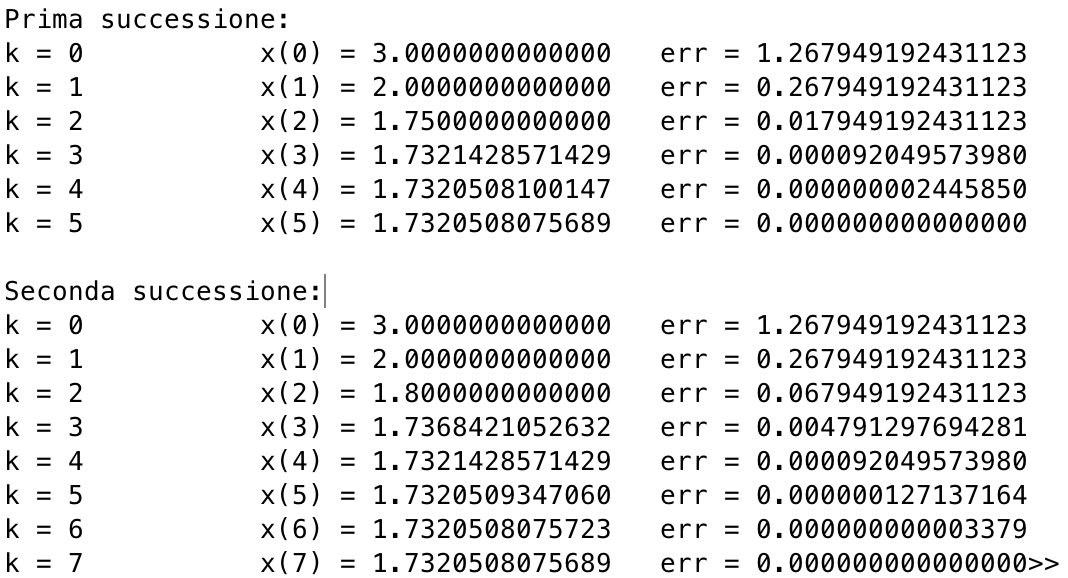
\includegraphics[width=12cm]{Capitolo1/es1_6.png}

	\end{flushleft}

\chapter{Esercizi A.A. 2017-18}

\markboth{CAPITOLO 2. ESERCIZI A.A. 2017-18}{CAPITOLO 2. ESERCIZI A.A. 2017-18}
\begin{flushleft}
	\textbf{Esercizio 2.1} \textit{Determinare analiticamente gli zeri del polinomio}\\
	\begin{center}
		$P(x) = x^3 - 4x^2 + 5x - 2$
	\end{center}
	\textit{e la loro molteplicit�. Dire perch� il metodo di bisezione � utilizzabile per approssimarne uno a partire dall'intervallo di confidenza $[a, b] = [0, 3]$. A quale zero di P potr� tendere la successione generata dal metodo di bisezione a partire da tale intervallo? Costruire una tabella in cui si riportano il numero di iterazioni e di valutazioni di P richieste per valori decrescenti della tolleranza} tolx.\\
	\medskip
	\textbf{Soluzione:} Prendiamo in considerazione il nostro polinomio e vediamo subito che un suo zero � 1, infatti:\\
	con $\hat{x} = 1:$
	\begin{center}
		$P(1) = 1^3 -4*1^2 +5*1 - 2 =$\\
		$= 1 - 4 + 5 - 2 = 0$
	\end{center}
	A questo punto controlliamo la sua molteplicit�:
	\begin{center}
		$P'(x) = 3x^2 - 8x + 5$\\
		$P'(1) = 3 - 8 + 5 = 0$\\
		\medskip
		$P''(x) = 6x - 8$\\
		$P''(1) = 6 - 8 = -2$
	\end{center}
	La molteplicit� � 2 poich� la derivata seconda � la prima derivata in ordine che non viene annullata.\\
	\medskip
	Un'altro suo zero � 2:\\
	con $\hat{x} = 2:$
	\begin{center}
		$P(2) = 8 - 16 + 10 - 2 = 0$
	\end{center}
	\begin{center}
		$P'(2) = 12 - 16 + 5 = 1$
	\end{center}
	In questo caso la molteplicit� � 1.\\
	\medskip
	Il metodo di bisezione � utilizzabile nell'intervallo di confidenza $[0, 3]$ in quanto $P(a)P(b)<0$, precisando che in tale intervallo P tender� a 2:\\
	\begin{center}
		$P(0) = 0 - 0 + 0 - 2 = -2$\\
		$P(3) = 27 - 36 + 15 - 2 = 4$\\
		$-2 * 4 < 0$\\
	\end{center}
	\newpage{}
	Di seguito i risultati dell'esecuzione del metodo di bisezione utilizzando come intervallo di confidenza $[0, 3]$:\\
	\begin{center}
		\begin{tabular}{|c|c|c|}
			\hline
			\multicolumn{3}{|c|}{$P(x) = x^3 - 4x^2 + 5x -2$, $\qquad I=\left[0,3\right]$}\tabularnewline
			\hline
			\multicolumn{3}{|c|}{$\tilde{x}{\ensuremath{\approx}}2.0$}\tabularnewline
			\hline
			$tol_{x}$ & Approssimazione & Iterazioni\tabularnewline
			\hline
			$10^{-1}$	& $\tilde{x} = 2.062500000000000$ &	$i = 3$\tabularnewline
			\hline
			$10^{-2}$ &	$\tilde{x} = 1.992187500000000$ & $i = 6$\tabularnewline
			\hline
			$10^{-3}$ &	$\tilde{x} = 2.000976562500000$ & $i = 9$\tabularnewline
			\hline
			$10^{-4}$ &	$\tilde{x} = 2.000061035156250$ & $i = 13$\tabularnewline
			\hline
			$10^{-5}$ &	$\tilde{x} = 1.999992370605469$ & $i = 16$\tabularnewline
			\hline
			$10^{-6}$ &	$\tilde{x} = 2.000000953674316$ & $i = 19$\tabularnewline
			\hline
			$10^{-7}$ &	$\tilde{x} = 2.000000059604645$ & $i = 23$\tabularnewline
			\hline
			$10^{-8}$ &	$\tilde{x} = 1.999999992549419$ & $i = 26$\tabularnewline
			\hline
			$10^{-9}$ &	$\tilde{x} = 2.000000000931323$ & $i = 29$\tabularnewline
			\hline
			$10^{-10}$ & $\tilde{x} = 2.000000000058208$ &	$i = 33$\tabularnewline
			\hline
			$10^{-11}$ & $\tilde{x} = 1.999999999992724$ &	$i = 36$\tabularnewline
			\hline
			$10^{-12}$ & $\tilde{x} = 2.000000000000909$ &	$i = 39$\tabularnewline
			\hline
			$10^{-13}$ & $\tilde{x} = 2.000000000000057$ &	$i = 43$\tabularnewline
			\hline
			$10^{-14}$ & $\tilde{x} = 1.999999999999993$ &	$i = 46$\tabularnewline
			\hline
			$10^{-15}$ & $\tilde{x} = 2.000000000000001$ &	$i = 49$\tabularnewline
			\hline
		\end{tabular}
	\end{center}
	Notiamo come dopo 49 iterazioni otteniamo il risultato con tolleranza pari a $10^{-15}$.\\
	\newpage
	\textbf{Esercizio 2.2} \textit{Completare la tabella precedente riportando anche il numero di iterazioni e di valutazioni di P richieste dal metodo di Newton, dal metodo delle corde e dal metodo delle secanti (con secondo termine della successione ottenuto con Newton) a partire dal punto $x_{0} = 3$. Commentare i risultati riportati in tabella. E' possibile utilizzare $x_{0} = 5/3$ come punto di innesco?}\\
	\textbf{Soluzione:}
	\begin{center}
		\begin{tabular}{|c|c|c|c|}
			\hline
			\multicolumn{4}{|c|}{$P(x) = x^3 - 4x^2 + 5x -2$, \qquad $x_{0} = 3$}\tabularnewline
			\hline
			\multicolumn{4}{|c|}{$\tilde{x}{\ensuremath{\approx}}2.0$}\tabularnewline
			\hline
			$tol_{x}$ & Newton & Corde & Secanti\tabularnewline
			\hline
			$10^{-1}$ & $\tilde{x} = 2.00435, i = 4$ & $x = 2.35938, i = 3$ & $x = 2.05016, i = 4$\tabularnewline
			\hline
			$10^{-2}$ & $\tilde{x} = 2.00004, i = 5$ & $x = 2.06432, i = 13$ & $x = 2.00099, i = 6$\tabularnewline
			\hline
			$10^{-3}$ & $\tilde{x} = 2.00000, i = 6$ & $x = 2.00767, i = 29$ & $x = 2.00002, i = 7$\tabularnewline
			\hline
			$10^{-4}$ & $\tilde{x} = 2.00000, i = 6$ & $x = 2.00078, i = 47$ & $x = 2.00000, i = 8$\tabularnewline
			\hline
			$10^{-5}$ & $\tilde{x} = 2.00000, i = 7$ & $x = 2.00007, i = 66$ & $x = 2.00000, i = 9$\tabularnewline
			\hline
			$10^{-6}$ & $\tilde{x} = 2.00000, i = 7$ & $x = 2.00001, i = 84$ & $x = 2.00000, i = 9$\tabularnewline
			\hline
			$10^{-7}$ & $\tilde{x} = 2.00000, i = 7$ & $x = 2.00000, i = 102$	& $x = 2.00000, i = 9$\tabularnewline
			\hline
			$10^{-8}$ & $\tilde{x} = 2.00000, i = 7$ & $x = 2.00000, i = 120$ & $x = 2.00000, i = 10$\tabularnewline
			\hline
			$10^{-9}$ & $\tilde{x} = 2.00000, i = 8$ & $x = 2.00000, i = 139$ & $x = 2.00000, i = 10$\tabularnewline
			\hline
			$10^{-10}$ & $\tilde{x} = 2.00000, i = 8$ & $x = 2.00000, i = 157$ & $x = 2.00000, i = 10$\tabularnewline
			\hline
			$10^{-11}$ & $\tilde{x} = 2.00000, i = 8$ & $x = 2.00000, i = 175$ & $x = 2.00000, i = 10$\tabularnewline
			\hline
			$10^{-12}$ & $\tilde{x} = 2.00000, i = 8$ & $x = 2.00000, i = 193$ & $x = 2.00000, i = 11$\tabularnewline
			\hline
			$10^{-13}$ & $\tilde{x} = 2.00000, i = 8$ & $x = 2.00000, i = 211$ & $x = 2.00000, i = 11$\tabularnewline
			\hline
			$10^{-14}$ & $\tilde{x} = 2.00000, i = 8$ & $x = 2.00000, i = 230$ & $x = 2.00000, i = 11$\tabularnewline
			\hline
			$10^{-15}$ & $\tilde{x} = 2.00000, i = 8$ & $x = 2.00000, i = 247$ & $x = 2.00000, i = 11$\tabularnewline
			\hline
		\end{tabular}
	\end{center}
	Possiamo notare come il metodo pi� efficiente � quello di Newton, mentre il metodo meno efficiente � quello delle corde.\\
	No non � possibile utilizzare $x_{0} = 5/3$ come punto di innesco in quanto $5/3$ � uno zero della derivata prima.\\
	\medskip
	\newpage
	\textbf{Esercizio 2.3} \textit{Costruire una seconda tabella analoga alla precedente relativa ai metodi di Newton, di Newton modificato e di accelerazione di Aitken applicati alla funzione polinomiale P a partire dal punto di innesco $x_{0} = 0$. Commentare i risultati riportati in tabella.}\\
	\medskip
	\textbf{Soluzione:}
	Avendo valutato precedentemente che la molteplicit� di P � 2 applichiamo il metodo di Newton modificaton con coefficente del termine di correzione $m = 2$:
	\begin{center}
		\begin{tabular}{|c|c|c|c|}
			\hline
			\multicolumn{4}{|c|}{$P(x) = x^3 - 4x^2 + 5x -2$, \qquad $x_{0} = 0$}\tabularnewline
			\hline
			\multicolumn{4}{|c|}{$\tilde{x}{\ensuremath{\approx}}1.0$}\tabularnewline
			\hline
			$tol_{x}$ & Newton & Newton modificato & Aitken\tabularnewline
			\hline
			$10^{-1}$ & $\tilde{x} = 0.89599, i = 4$ & $x = 0.99607, i = 3$ & $x = 1.00056, i = 3$\tabularnewline
			\hline
			$10^{-2}$ & $\tilde{x} = 0.99289, i = 8$ & $x = 0.99999, i = 4$ & $x = 1.00000, i = 4$\tabularnewline
			\hline
			$10^{-3}$ & $\tilde{x} = 0.99911, i = 11$ & $x = 1.00000, i = 5$ & $x = 1.00000, i = 4$\tabularnewline
			\hline
			$10^{-4}$ & $\tilde{x} = 0.99994, i = 15$ & $x = 1.00000, i = 5$ & $x = 1.00000, i = 5$\tabularnewline
			\hline
			$10^{-5}$ & $\tilde{x} = 0.99999, i = 18$ & $x = 1.00000, i = 5$ & $x = 1.00000, i = 5$\tabularnewline
			\hline
			$10^{-6}$ & $\tilde{x} = 1.00000, i = 21$ & $x = 1.00000, i = 6$ & $x = 1.00000, i = 5$\tabularnewline
			\hline
			$10^{-7}$ & $\tilde{x} = 1.00000, i = 25$ & $x = 1.00000, i = 6$	& $x = 1.00000, i = 5$\tabularnewline
			\hline
			$10^{-8}$ & $\tilde{x} = 1.00000, i = 29$ & $x = 1.00000, i = 6$ & $x = 1.00000, i = 6$\tabularnewline
			\hline
			$10^{-9}$ & $\tilde{x} = 1.00000, i = 29$ & $x = 1.00000, i = 6$ & $x = 1.00000, i = 6$\tabularnewline
			\hline
			$10^{-10}$ & $\tilde{x} = 1.00000, i = 29$ & $x = 1.00000, i = 6$ & $x = 1.00000, i = 6$\tabularnewline
			\hline
			$10^{-11}$ & $\tilde{x} = 1.00000, i = 29$ & $x = 1.00000, i = 6$ & $x = 1.00000, i = 6$\tabularnewline
			\hline
			$10^{-12}$ & $\tilde{x} = 1.00000, i = 29$ & $x = 1.00000, i = 6$ & $x = 1.00000, i = 6$\tabularnewline
			\hline
			$10^{-13}$ & $\tilde{x} = 1.00000, i = 29$ & $x = 1.00000, i = 6$ & $x = 1.00000, i = 6$\tabularnewline
			\hline
			$10^{-14}$ & $\tilde{x} = 1.00000, i = 29$ & $x = 1.00000, i = 6$ & $x = 1.00000, i = 6$\tabularnewline
			\hline
			$10^{-15}$ & $\tilde{x} = 1.00000, i = 29$ & $x = 1.00000, i = 6$ & \tabularnewline
			\hline
		\end{tabular}
	\end{center}
	Come era prevedibile notiamo che il metodo di Newton converge linearmente. Il metodo di Newton modificato e quello di Aitken performano similmente e notiamo che il costo di discosta di poco.\\
\newpage
\textbf{Esercizio 2.4} \textit{Definire una procedura iterativa basata sul metodo di Newton per approssimare \(\sqrt\alpha \), per un assegnato \(\alpha > 0\). Costruire una tabella dove si riportano le successive approssimazioni ottenute e i corrispondenti errori assoluti (usare l'approssimazione di Matlab di \(\sqrt\alpha \) per il calcolo dell'errore) nel caso in cui \(\alpha=5\) partendo da \(x_0=5\).}\\
\textbf{Soluzione:}
Il seguente metodo produrr� la tabella richiesta:
\lstinputlisting[language=Matlab]{Capitolo2/es2_4.m}
\begin{center}
	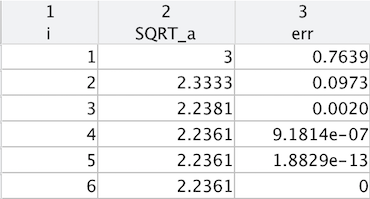
\includegraphics[scale=1]{Capitolo2/es2_4.png}
\end{center}
\newpage
\textbf{Esercizio 2.5} \textit{
Definire una procedura iterativa basata sul metodo delle secanti sempre per approssimare \(\sqrt\alpha \), per un assegnato \(\alpha > 0\). Completare la tabella precedente aggiungendovi i risultati ottenuti con tale precedura partendo da \(x_0=5\) e \(x_1=3\). Commentare i risultati riportati in tabella.}\\
\textbf{Soluzione:}
\lstinputlisting[language=Matlab]{Capitolo2/es2_5.m}
\begin{center}
	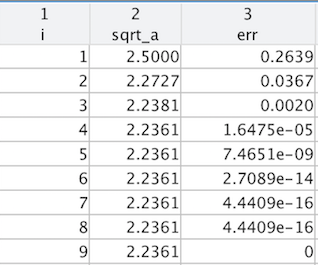
\includegraphics[scale=1]{Capitolo2/es2_5.png}
\end{center}
Dal risultato ottenuto possiamo notare come a differenza del metodo di newton il metodo delle secanti converge \(\sqrt\alpha \) meglio nelle prime iterazioni, ma il metodo di Newton converge poi con pi� precisione convergendo pi� velocemente verso il risultato esatto.\\
\newpage
\end{flushleft}

\chapter{Esercizi A.A. 2017-18}
\markboth{CAPITOLO 3. ESERCIZI A.A. 2017-18}{CAPITOLO 3. ESERCIZI A.A. 2017-18}
\begin{flushleft}
\textbf{Esercizio 3.1} \textit{Scrivere una function Matlab per la risoluzione di un sistema lineare con matrice dei coefficienti triangolare inferiore a diagonale unitaria. Inserire un esempio di utilizzo.}\\
\textbf{Soluzione: }
\lstinputlisting[language=Matlab]{Capitolo3/es3_1.m}
Il codice risolve sistemi lineari con matrice dei coefficenti triangolare inferiore a diagonale unitaria dove in input viene presa la matrice dei coefficienti \(A\) e il vettore dei termini noti \(b\) restituendo  vettore con le soluzioni.\\
Un esempio � il seguente:
\[
\begin{bmatrix}1 & 0 & 0 \\ 3 & 1 & 0\\ 4 & 1 & 2 \end{bmatrix} \bar{x} = \begin{bmatrix}1 \\ 2 \\ 3 \end{bmatrix}
\]
Il vettore delle soluzioni calcolato dalla funzione �: \(\begin{bmatrix}1 & -1 & 0 \end{bmatrix}\).\\
\bigskip
\textbf{Esercizio 3.2} \textit{Utilizzare l'Algoritmo 3.6 del libro per stabilire se le seguenti matrici sono sdp o no,}

\[
A_1 = \begin{pmatrix}1 & -1 & 2 & 2 \\ -1&5&-14&2\\ 2&-14&42&2\\2&2&2&65 \end{pmatrix},
A_2 = \begin{pmatrix}1 & -1 & 2 & 2 \\ -1&6&-17&3\\ 2&-17&48&-16\\2&3&-16&4 \end{pmatrix}
\]

\textbf{Soluzione: }Il seguente codice implementa l'algoritmo richiesto e si evince che la matrice $A_{1}$ � simmetrica e difinita positiva mentre la matrice $A_{2}$ non lo �:\\
\newpage
\lstinputlisting[language=Matlab]{Capitolo3/es3_2.m}
\bigskip
\textbf{Esercizio 3.3}
\textit{Scrivere una function Matlab che, avendo in ingresso un vettore b contenente i termini noti del sistema lineare \(Ax = b\) con \textit{A} sdp e l'output dell'Algoritmo 3.6 del libro (matrice \(A\) riscritta nella porzione triangolare inferiore con i fattori \(L\) e \(D\) della fattorizzazione \(LDL^T\) di \(A\)), ne calcoli efficientemente la soluzione.}\\
\textbf{Soluzione: }
\lstinputlisting[language=Matlab]{Capitolo3/es3_3.m}
La function \lstinline[language=Matlab]{sistema_triang_inf} � stata implementata nell'esercizio 1 di questo capitolo.\\
\bigskip
\textbf{Esercizio 3.4} \textit{Scrivere una function Matlab che, avendo in ingresso un vettore b contenente i termini noti del sistema lineare \(Ax = b\)  e l'output dell'Algoritmo 3.7 del libro (matrice \(A\) riscritta con la fattorizzazione LU con pivoting parziale e il vettore p delle permutazioni), ne calcoli efficientemente la soluzione.}\\
\textbf{Soluzione: }
Il seguente codice calcola quanto richiesto, le function \lstinline[language=Matlab]{sistema_triang_inf} e \lstinline[language=Matlab]{sistema_triang_sup} sono quelle degli Esercizi 1 e 3.\\
\lstinputlisting[language=Matlab]{Capitolo3/es3_4.m}
\bigskip
\textbf{Esercizio 3.5} \textit{Inserire alcuni esempi di utilizzo delle due function implementate per i punti 3 e 4, scegliendo per ciascuno di essi un vettore \(\hat{x}\) e ponendo \(b = A\hat{x}\). Riportare \(\hat{x}\) e la soluzione \(x\) da essi prodotta. Costruire anche una tabella in cui, per ogni esempio considerato, si riportano il numero di condizionamento di A in norma 2 (usare \textbf{cond} di Matlab) e le quantit� \(||r||/||b||\) e \(||x-\hat{x}||/||\hat{x}||\).}\\
\textbf{Soluzione: } Per dimostrare le function dell'esercizio 3 (risoluzione di sistemi $LDL^T$) e dell'esercizio 4 (scomposizione LU con pivoting parziale) verr� utilizzata la seguente matrice:\\
\[
A = \begin{pmatrix} 1 & -1 & 2 & 2 \\ -1 & 5 & -14 & 2\\ 2 & -14 & 42 & 2\\ 2 & 2 & 2 & 65 \end{pmatrix}
\]
\noindent I vettori scelti sono, rispettivamente per svolgere gli esercizi 3 e 4:

\[
\hat{x}_3 = \begin{bmatrix} 5.1211 \\ 3.4433 \\ 0.1257 \\ 2.1579 \end{bmatrix},
\hat{x}_4 = \begin{bmatrix} 1.3345 \\ 2.3232 \\ 3.1175 \\ 1.6658 \end{bmatrix}
\]

\noindent Ponendo \(b=A\hat{x}\) risulter� rispettivamente:
\\
\[
b_3 = \begin{bmatrix} 6.2450 \\ 14.6514 \\ -28.3688 \\ 157.6437 \end{bmatrix},
b_4 = \begin{bmatrix} 8.5779 \\ -30.0319 \\ 104.4108 \\ 121.8274 \end{bmatrix}
\]

\noindent Eseguendo le function create per la risoluzione del sistema viene generata la seguente soluzione:

\[
x_3 = \begin{bmatrix} 5.12110000000000 \\ 3.44330000000000 \\ 0.125699999999998 \\ 2.15790000000000 \end{bmatrix},
x_4 = \begin{bmatrix} 1.33450000000002 \\ 2.32320000000003 \\ 3.11750000000001 \\ 1.66580000000000 \end{bmatrix}
\]
\\
\noindent La tabella seguente mostra il condizionamento della matrice restituita dagli algoritmi di fattorizzazione ed i vari confronti di errori relativi sui dati di ingresso (\(||r||/||b||\)) e sul risultato (\(||x-\hat{x}||/||\hat{x}||\)):
\bigskip{}
\noindent\begin{tabular}{l*{20}{c}}
Fattorizzazione & \vline& \(\hat{x}\) & \vline& \(cond(A, 2)\) & \vline& \(||r||/||b||\) & \vline& \(||x-\hat{x}||/||\hat{x}||\) \\
\hline
\(LDL^T\)    & \vline& \(\hat{x}_3\) & \vline& \(3.6158 \times 10^3\) & \vline& \(4.4142 \times 10^{-17}\)	& \vline& \(8.3347 \times 10^{-16}\)   \\
\(LU\) pivot & \vline& \(\hat{x}_4\) & \vline& 319.1025 & \vline& \(9.0270 \times 10^{-17}\)	& \vline& \(8.4115 \times 10^{-15}\) 	 \\

\end{tabular}
\\

\noindent Il codice Matlab usato per realizzare i precedenti esempi � il seguente:\\
\lstinputlisting[language=Matlab]{Capitolo3/es3_5.m}
\bigskip{}
\textbf{Esercizio 3.6} \textit{Sia \(A = \begin{pmatrix} \epsilon & 1 \\ 1 & 1 \end{pmatrix}\) con $\epsilon=10^{-13}$.  Definire L triangolare inferiore a diagonale unitaria e U triangolare superiore in modo che il prodotto LU sia la fattorizzazione LU di A e, posto \(b=Ae\) con \(e=(1,1)^{T}\), confrontare l'accuratezza della soluzione che si ottiene usando il comando \(U \textbackslash (L \textbackslash b)\) (Gauss senza pivoting) e il comando \(A \textbackslash b\) (Gauss con pivoting).}\\
\textbf{Soluzione: }
Data la matrice A possiamo scrivere:\\
			\begin{center}
				$ A = L \times U =
				\begin{bmatrix}
				1 & 0 \\
				10^{13} & 1
				\end{bmatrix}
				\times
				\begin{bmatrix}
				10^{-13} & 1 \\
				0 & 1 - 10^{13}
				\end{bmatrix} $ \\
			\end{center}

			\lstinputlisting[language = matlab]{Capitolo3/es3_6.m}
			\noindent Calcoliamo \(b\):

			\[b = Ae = \begin{pmatrix} \epsilon & 1 \\ 1 & 1 \end{pmatrix} \begin{bmatrix} 1 \\ 1\end{bmatrix} = \begin{bmatrix} \approx 1 \\ 2 \end{bmatrix}\]
			\[U \textbackslash (L \textbackslash b) = \begin{bmatrix} 0.992 \\ 1\end{bmatrix}\]
			\[A \textbackslash b = \begin{bmatrix} 1 \\ 1\end{bmatrix}\]

			Dai calcoli richiesti segue che :\\
			\begin{center}
				$\varepsilon_{U \setminus (L \setminus b)} = 5.6517 \cdot 10^{-4}$ \hspace{10 pt} ed \hspace{10 pt} $ \varepsilon_{A \setminus b} = 2.2204 \cdot 10^{-16}$ \\
			\end{center}
			\noindent Si nota che il vettore \(b\) calcolato col metodo di Gauss senza pivoting abbia un'accuratezza minore rispetto alla sua versione calcolata con il metodo di Gauss con pivoting.
			\\
\bigskip
\textbf{Esercizio 3.7} \textit{Scrivere una function Matlab specifica per la risoluzione di un sistema lineare con matrice dei coefficienti \(A \in R^{n \times n}\) bidiagonale inferiore a diagonale unitaria di Toeplitz, specificabile con uno scalare \(\alpha\). Sperimentarne e commentarne le prestazioni (considerare il numero di condizionamento della matrice) nel caso in cui \(n=12\) e \(\alpha=100\) ponendo dapprima \(b=(1, 101, \ldots, 101)^T\) (soluzione esatta \(\hat{x}=(1,\ldots ,1)^T\)) e quindi \(b=0.1 * (1, 101, \ldots, 101)^T\) (soluzione esatta \(\hat{x}=(0.1,\ldots ,0.1)^T\)).}\\
\medskip
\textbf{Soluzione: } \noindent Ricordando che le matrici bidiagonali inferiori a diagonale unitaria di Toeplitz sono le matrici \(A \in R^{n \times n}\) del tipo \[\begin{pmatrix} 1 & 0 & 0 & \cdots & 0 \\ \alpha & 1 & 0 & \cdots & 0 \\ 0 & \alpha & 1 & \cdots & 0 \\ \vdots & \vdots & \vdots & \vdots & \vdots \\ 0 & \cdots & 0 & \alpha & 1\end{pmatrix}\]
\lstinputlisting[language=Matlab]{Capitolo3/es3_7.m}
Il seguente codice seguente applica le due function appena mostrate calcolando il condizionamento del problema e la soluzione nei due casi richiesti con $n = 12$ e $\alpha = 100$:\\
\lstinputlisting[language=Matlab]{Capitolo3/es3_7_esempio.m}
Il numero di conzionamento risulta essere infinito.
Di seguito vengono mostrati i risultati ottenuti nel primo caso e nel secondo caso relative a $x_{1}$ e $x_{2}$:
\[
x_1=\begin{bmatrix} 1 \\1\\1\\1\\1\\1\\1\\1\\1\\1\\1\\1\end{bmatrix}^T\qquad x_2=\begin{bmatrix}0.1000\\ 0.1000 \\ 0.1000 \\ 0.1000 \\ 0.1000 \\ 0.1000 \\ 0.1000 \\ 0.1014 \\ -0.0407 \\ 14.1702 \\ -1.4069 \times 10^3 \\ 1.4070 \times 10^5 \end{bmatrix}^T
\]\\
\bigskip
\textbf{Esercizio 3.8} \textit{Scrivere una function che, dato un sistema lineare sovradeterminato Ax = b, con \(A \in R^{m \times n}\), \(m > n\), \(rank(A)=n\) e \(b \in R^m\), preso come input b e l'output dell'Algoritmo 3.8 del libro (matrice A riscritta con la parte significativa dei vettori di Householder normalizzati con prima componente unitaria), ne calcoli efficientemente la soluzione nel senso dei minimi quadrati.}\\
\textbf{Soluzione: }
\lstinputlisting[language=Matlab]{Capitolo3/es3_8.m}
\bigskip
\textbf{Esercizio 3.9} \textit{Inserire due esempi diutilizzo della function implementata per il punto 8 e confrontare la soluzione ottenuta con quella fornita dal comando \(A \textbackslash b\).}\\
\textbf{Soluzione: }Per il primo esempio utilizzeremo:\\
\[
A_1 = \begin{pmatrix} 4 & 2 & 2 \\ 1 & 1& 2 \\ 2 & 3 & 4 \\ 2 & 1 & 1 \end{pmatrix} \quad b_1 = \begin{bmatrix} 4\\5\\4\\1 \end{bmatrix}
\]\\
La funzione restituisce:
\[
	x_{1} = \begin{bmatrix}1.533333333333334 \\ -5.99999999999999\\ 4.73333333333333 \end{bmatrix}^T \qquad e \qquad A_{1}\textbackslash b_{1} = \begin{bmatrix}1.53333333333333 \\ -6.00000000000000 \\ 4.73333333333333 \end{bmatrix}^T
\]\\
Per il secondo esempio invece:
\[
A_1 = \begin{pmatrix} 1 & 2 \\ 2 & 6 \\ 4 & 3 \end{pmatrix} \quad b_1 = \begin{bmatrix} 4\\5\\6 \end{bmatrix}
\]\\
La funzione restituisce:
\[
	x_{1} = \begin{bmatrix}1.15014164305949 \\ 0.532577903682720 \end{bmatrix}^T \qquad e \qquad A_{1}\textbackslash b_{1} = \begin{bmatrix}1.15014164305949 \\ 0.532577903682719 \end{bmatrix}^T
\]\\
In entrambi i casi $A\textbackslash b \approx x$\\
Il codice Matlab:
\lstinputlisting[language=Matlab]{Capitolo3/es3_9.m}
\bigskip
\textbf{Esercizio 3.10} \textit{Scrivere una function Matlab che realizza il metodo di Newton per un sistema nonlineare (prevedere un numero massimo di iterazioni e utilizzare il criteri di arresto basato sull'incremento in norma euclidea). Utilizzare la function costruita al punto 4 per la risoluzione del sistema lineare ad ogni iterazione.}\\
\textbf{Soluzione: }\lstinputlisting[language=Matlab]{Capitolo3/es3_10.m}
\bigskip
\textbf{Esercizio 3.11} \textit{Verificato che la funzione \(f(x_1,x_2) = x_1^2+x_2^3-x_1x_2\) ha un punto di minimo relativo in (1/12, 1/6), costruire una tabella in cui si riportano il numero di iterazioni eseguite, e la norma euclidea dell'ultimo incremento e quella dell'errore con cui viene approssimato il risultato esatto utilizzando la function sviluppata al punto precedente per valori delle tolleranze pari a \(10^{-t}\), con t = 3,6. Utilizzare (1/2, 1/2) come punto di innesco. Verificare che la norma dell'errore � molto pi� piccola di quella dell'incremento (come mai?)}\\
\textbf{Soluzione: }
\noindent Verifichiamo l'esistenza di un punto di minimo relativo in \((\frac{1}{12}, \frac{1}{6})\) considerando il sistema non lineare:
\[
F(\vec{x}) = \vec{0} \quad \text{con} \quad F = \begin{bmatrix}\frac{\partial}{\partial x_1}f(x_1,x_2) \\ \frac{\partial}{\partial x_2}f(x_1,x_2)  \end{bmatrix}
\]
\[
\frac{\partial}{\partial x_1}f(x_1,x_2) = 2x_1 -x_2 \quad \frac{\partial}{\partial x_2}f(x_1,x_2) = 3x_2^2 - x_1
\]
\[
\begin{cases}
2x_1 -x_2 = 0 \\
3y^2 - x_1 = 0
\end{cases}
\quad \text{ha come soluzioni} \quad \begin{bmatrix}0 & 0 \end{bmatrix} \quad \text{e} \quad \begin{bmatrix}\frac{1}{12} & \frac{1}{6}\end{bmatrix}
\]
\\
\noindent I punti trovati sono punti stazionari della funzione data.\\ Consideriamo la matrice Hessiana della funzione \(f(x,x_2)\), che coincide con la matrice Jacobiana della funzione \(F\):
\[
H =
\begin{bmatrix} f_{x_1x_1} & f_{x_1x_2} \\ f_{x_2x_1} & f_{x_2x_2} \end{bmatrix}
=
\begin{bmatrix} 2 & -1 \\ -1 & 6x_2 \end{bmatrix}
= J_F
\quad
\det(H) = 12x_2 - 1
\]

\noindent Il determinante della matrice Hessiana � positivo per \(x_2=\frac{1}{6}\), ed il primo elemento � positivo qui abbiamo un punto di minimo relativo in \((\frac{1}{12}, \frac{1}{6})\).
\\
\bigskip
\noindent I seguenti dati sono stati ottenuti considerando come soluzione esatta \(\hat{x} = [\frac{1}{12}, \frac{1}{6}]\) e come ultimo incremento la quantit� \(||x^{(i)} - x^{(i-1)}||\):
\\

\[
\begin{tabular}{l*{15}{c}}
 Tolleranza & \vline& iterazioni & \vline& \(||x^{(i)} - x^{(i-1)}||\) & \vline& \(||x - \hat{x}||\) \\
\hline
 \(10^{-3}\) & \vline& 5 &\vline& 2.8369 \(\times 10^{-4}\) & \vline& 4.3190 \(\times 10^{-7}\) \\
 \(10^{-4}\) & \vline& 6 &\vline& 4.3190 \(\times 10^{-7}\) & \vline& 1.0011 \(\times 10^{-12}\) \\
 \(10^{-5}\) & \vline& 6 &\vline& 4.3190 \(\times 10^{-7}\) & \vline& 1.0011 \(\times 10^{-12}\) \\
 \(10^{-6}\) & \vline& 6 &\vline& 4.3190 \(\times 10^{-7}\) & \vline& 1.0011 \(\times 10^{-12}\) \\
\end{tabular}
\] \\
La norma dell'ultimo incremento sara' molto minore rispetto alla norma dell'errore di approssimanzione del risultato. Avendo che il metodo di Newton ha ordine di convergenza pari a 2, che consente all'approssimazione del risultato di convergere velocemente verso il risultato esatto.
\lstinputlisting[language=Matlab]{Capitolo3/es3_11.m}

\end{flushleft}

\chapter{Esercizi A.A. 2017-18}
\markboth{CAPITOLO 4. ESERCIZI A.A. 2017-18}{CAPITOLO 4. ESERCIZI A.A. 2017-18}
\begin{flushleft}
\textbf{Esercizio 4.1} \textit{Scrivere una function Matlab che implementi il calcolo del polinomio interpolante di grado \textit{n} in forma di Lagrange. \\La forma della function deve essere del tipo: \lstinline[language=Matlab]{Capitolo4/y = lagrange( xi, fi, x )}}\\
\textbf{Soluzione: } \lstinputlisting[language=Matlab]{Capitolo4/es4_1.m}
\bigskip
\textbf{Esercizio 4.2} \textit{Scrivere una function Matlab che implementi il calcolo del polinomio interpolante di grado \textit{n} in forma di Newton. \\La forma della function deve essere del tipo: \lstinline[language=Matlab]{Capitolo4/y = newton( xi, fi, x )}}\\
\textbf{Soluzione: } \lstinputlisting[language=Matlab]{Capitolo4/es4_2.m}
\bigskip
\textbf{Esercizio 4.3} \textit{Scrivere una function Matlab che implementi il calcolo del polinomio interpolante di Hermite. \\La forma della function deve essere del tipo: \lstinline[language=Matlab]{Capitolo4/y = hermite( xi, fi, f1i, x )}}\\
\textbf{Soluzione: }  \lstinputlisting[language=Matlab]{Capitolo4/es4_3.m}
\newpage
\textbf{Esercizio 4.4} \textit{Utilizzare le functions degli esercizi precedenti per disegnare l'approssimazione della funzione \(\sin(x)\) nell'intervallo \([0, 2\pi]\), utilizzando le ascisse di interpolazione \(x_i=i\pi\), \(i= 0,1,2\).}\\
\textbf{Soluzione: }
\begin{center}
	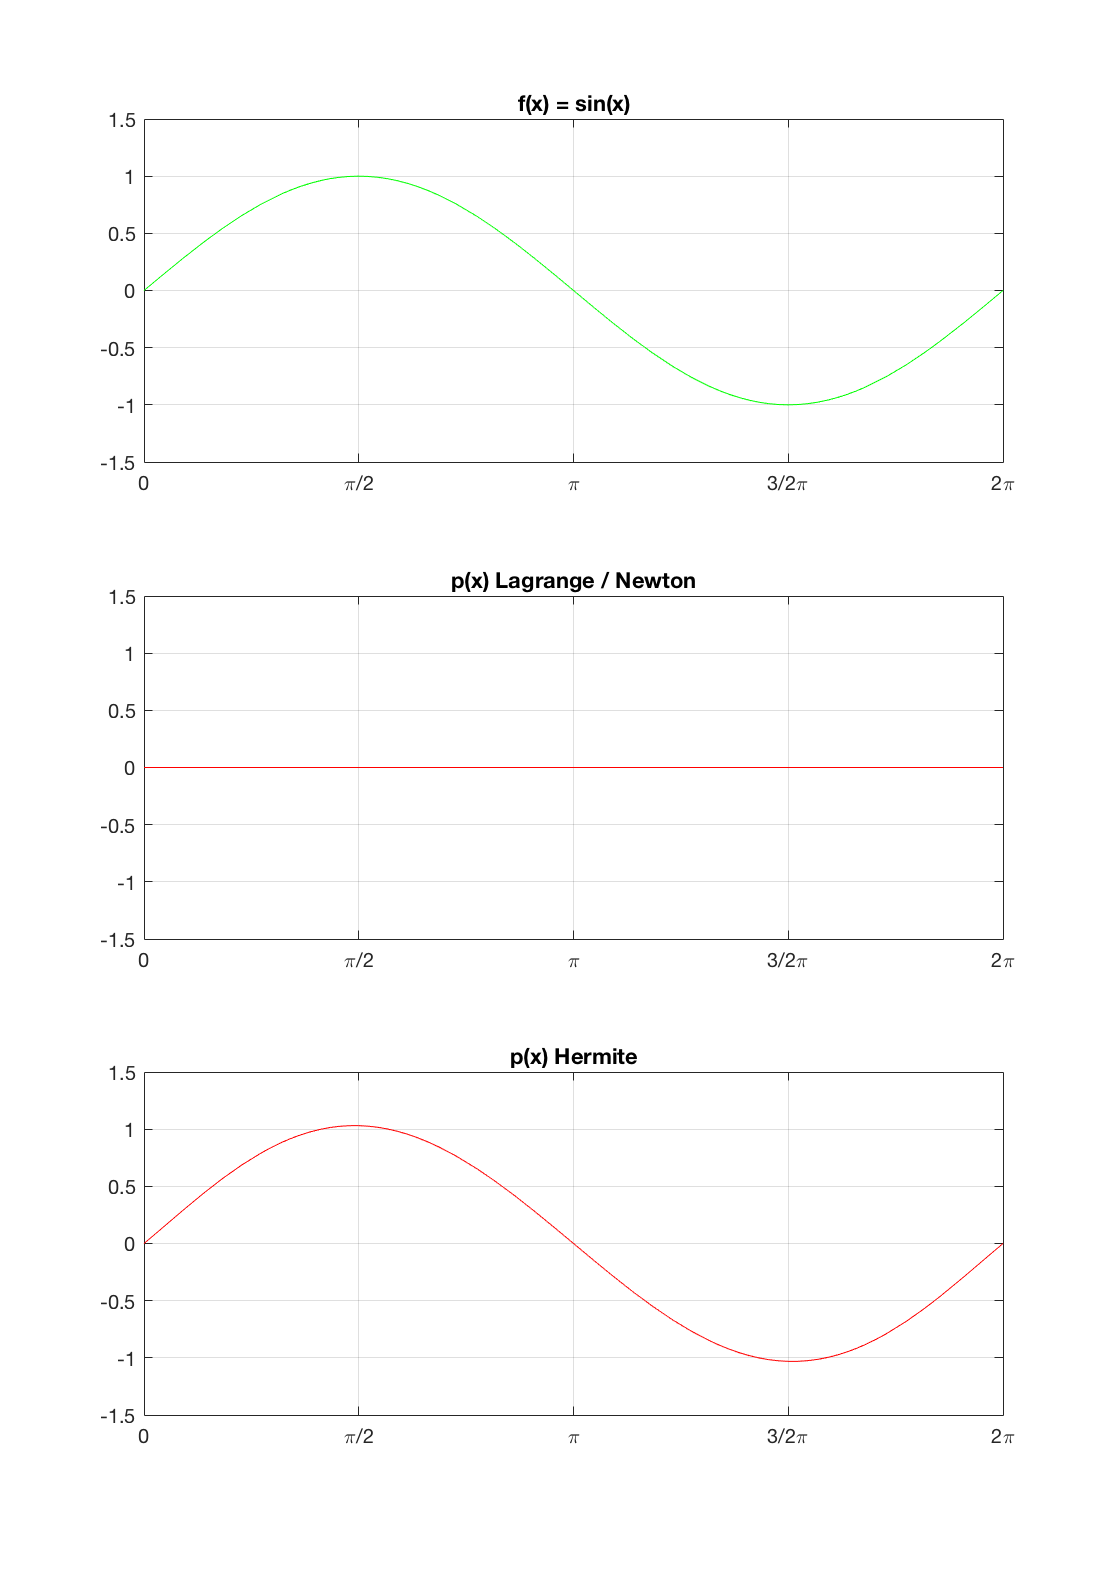
\includegraphics[scale=0.31]{Capitolo4/es4_4.png}
\end{center}
Possiamo notare come il polinomio di Lagrange e Newton genera una retta $y=0$ essendo $f_{i} = 0$ in tutte le ascisse.
\lstinputlisting[language=Matlab]{Capitolo4/es4_4.m}
\bigskip
\textbf{Esercizio 4.5} \textit{Scrivere una function Matlab che implementi la spline cubica interpolante (naturale o \textit{not-a-knot}, come specificato in ingresso) delle coppie di dati assegnate. La forma della funcion deve essere del tipo: \lstinline[language=Matlab]{Capitolo4/y = spline3(xi, fi, x, tipo)}}\\
\textbf{Soluzione: } Il seguente codice Matlab implementa la function richiesta. Per rendere il codice pi� leggibile sono state craete varie sottofunzioni.\\ Il codice � stato testato con un banale esempio:
\lstinputlisting[language=Matlab]{Capitolo4/es4_5.m}
\bigskip
\textbf{Esercizio 4.6} \textit{Scrivere una function Matlab che implementi il calcolo delle ascisse di Chebyshev per il polinomio interpolante di grado \textit{n}, su un generico intervallo \([a, b]\). \\La function deve essere del tipo: \lstinline[language=Matlab]{Capitolo4/ xi = ceby( n, a, b )}}\\
\textbf{Soluzione: }
\lstinputlisting[language=Matlab]{Capitolo4/es4_6.m}
\newpage
\textbf{Esercizio 4.7} \textit{Utilizzare le function degli Esercizi 4.1 e 4.6 per graficare l'approssimazione della funzione di Runge sull'intervallo \([-6, 6]\), per \(n = 2, 4, 6, \ldots, 40\). Stimare numericamente l'errore commesso in funzione del grado \textit{n} del polinomio interpolante.}\\
\textbf{Soluzione: } Di seguito i grafici che mostrano i polinomi interpolanti di grado \textit{n} calcolati utilizzando come punti di interpolazione quelli corrispondenti alle \textit{n} ascisse di Chebyshev, sovrapposti al grafico della funzione di Runge: \(f(x) = \frac{1}{1+x^2}\). \\
\begin{tabular}{c c}
\(n=2\) & \(n=4\) \\
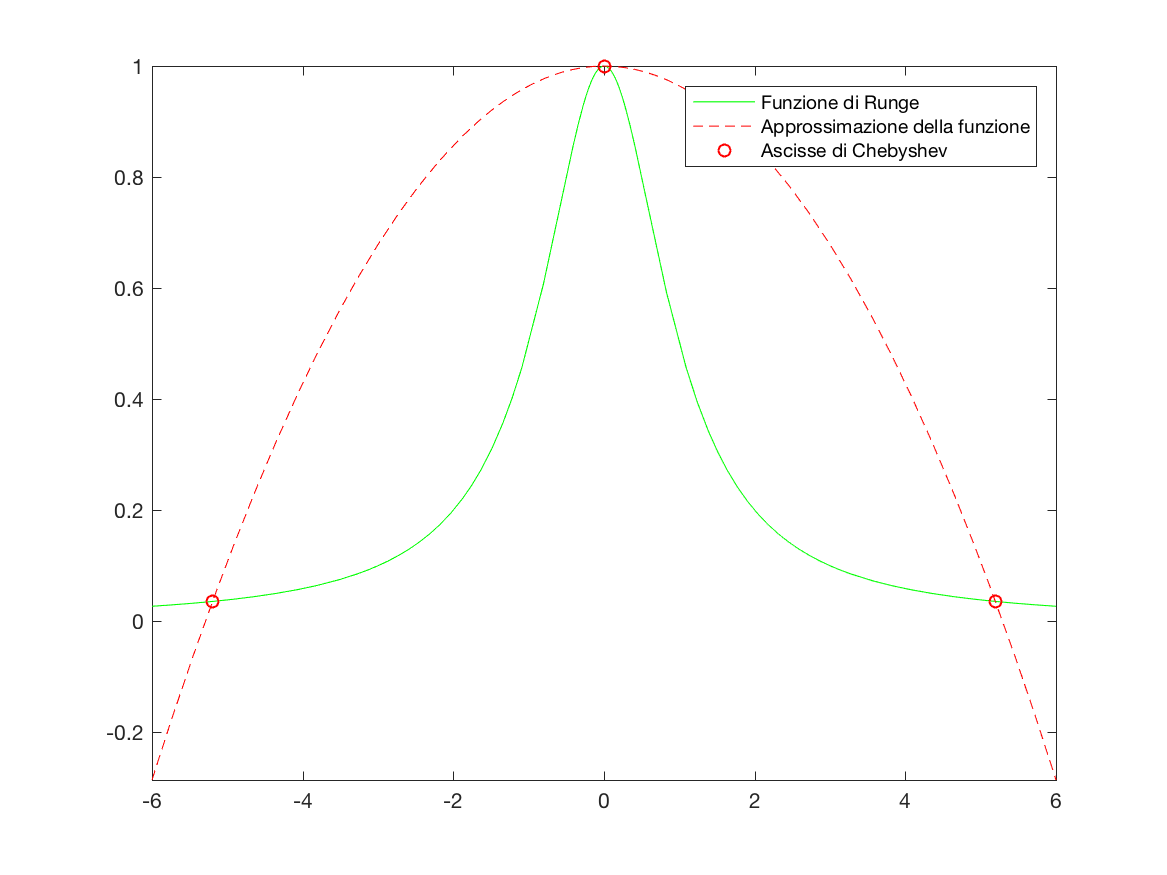
\includegraphics[scale=0.333]{Capitolo4/graficiEs7/es4_7_img2.png} &  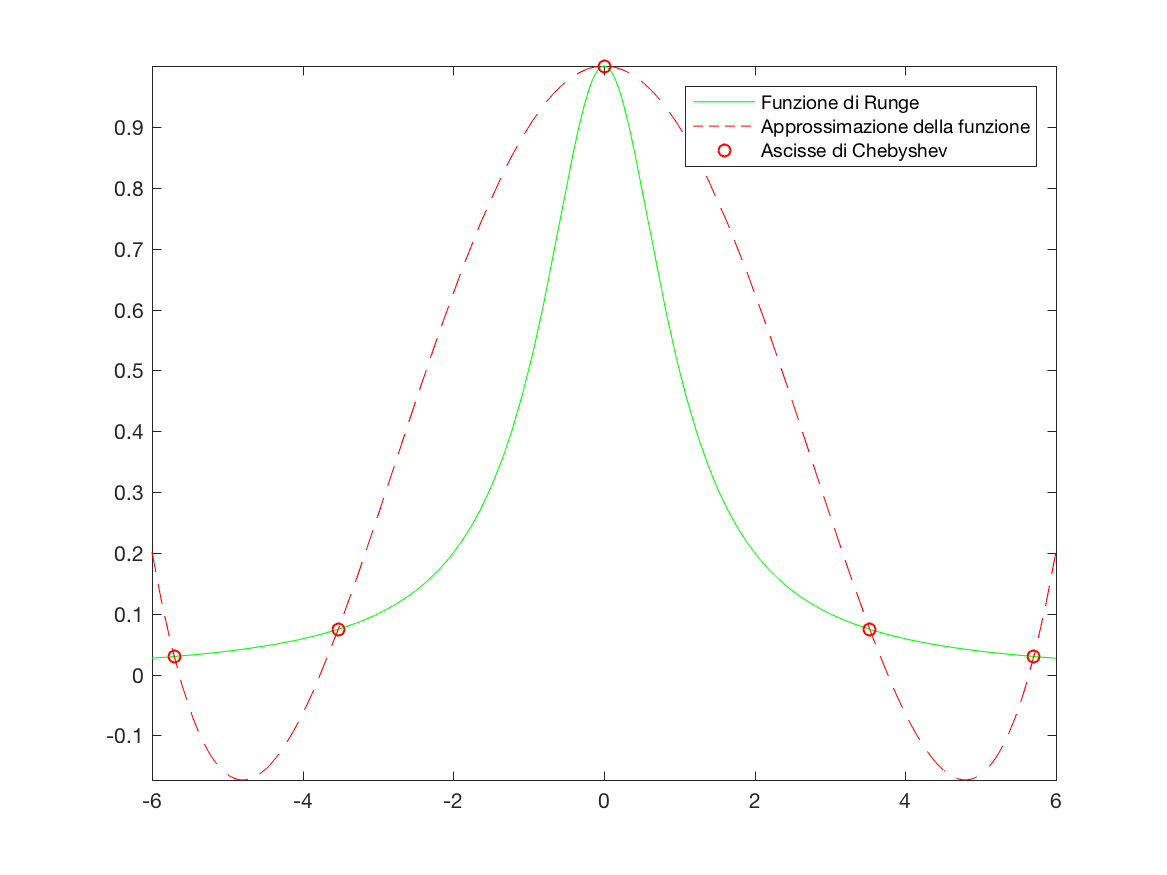
\includegraphics[scale=0.333]{Capitolo4/graficiEs7/es4_7_img4.png} \\
\(n=6\)& \(n=8\) \\
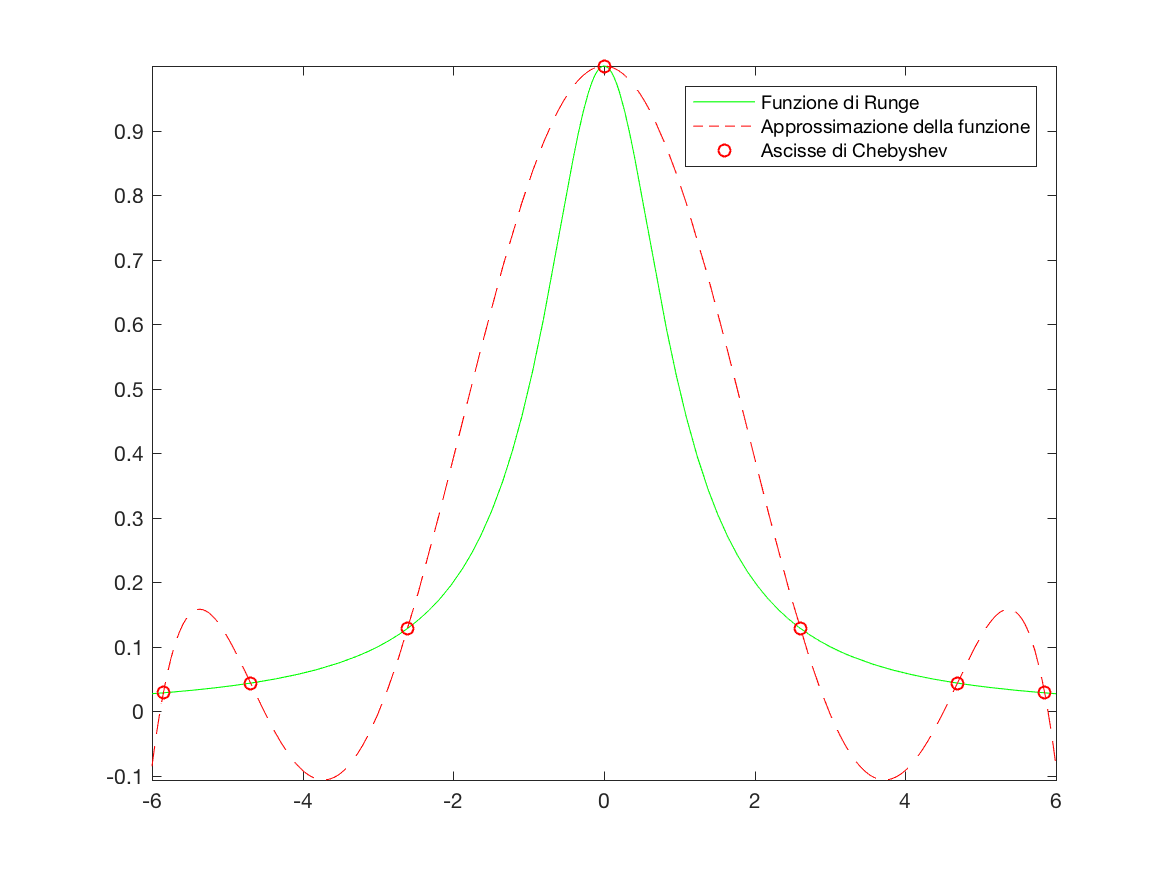
\includegraphics[scale=0.333]{Capitolo4/graficiEs7/es4_7_img6.png} &  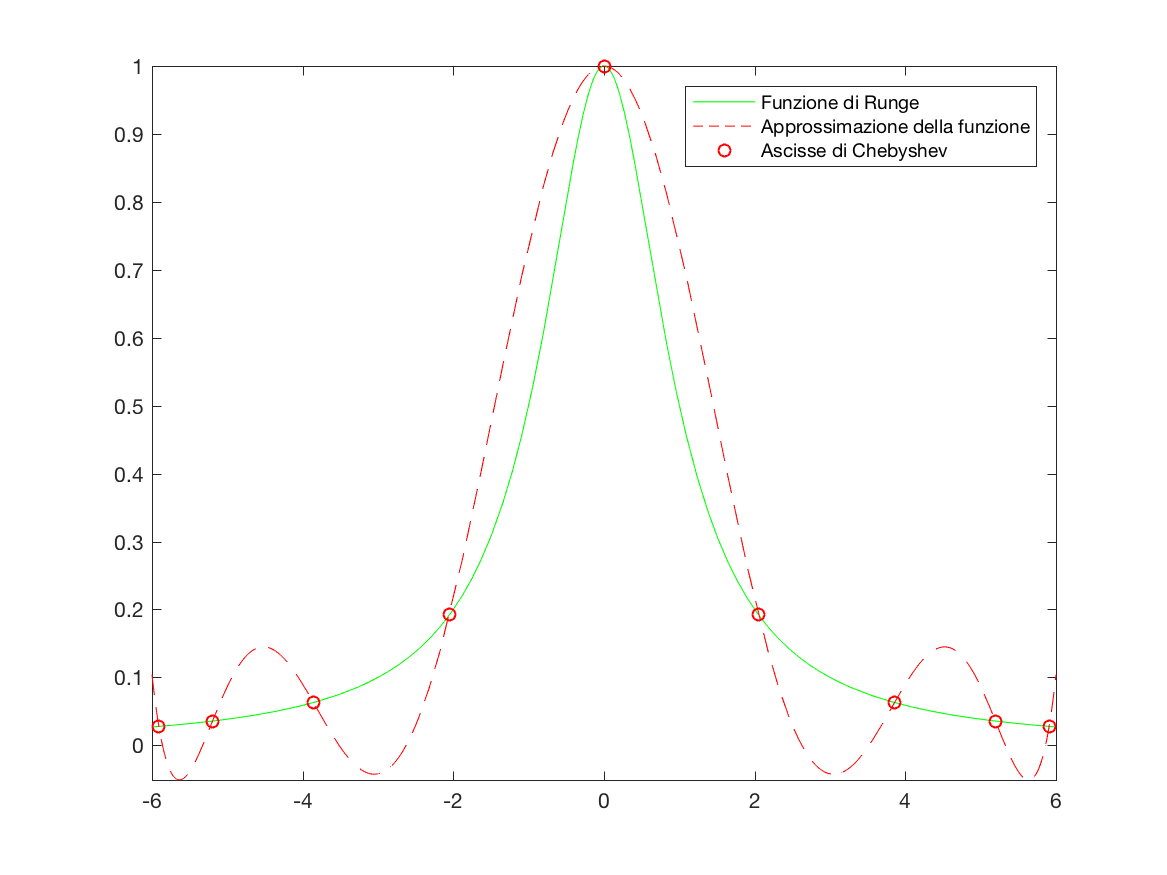
\includegraphics[scale=0.333]{Capitolo4/graficiEs7/es4_7_img8.png} \\
\(n=10\) &  \(n=12\) \\
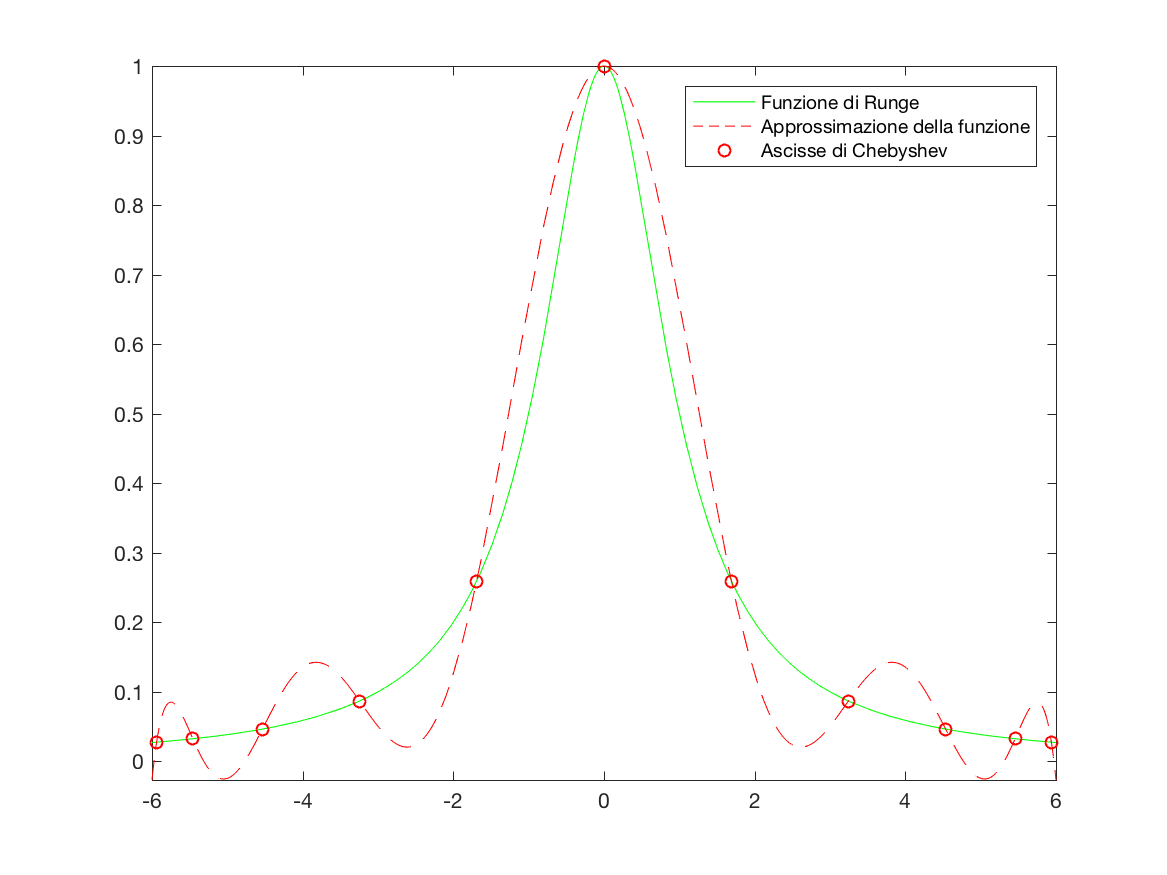
\includegraphics[scale=0.333]{Capitolo4/graficiEs7/es4_7_img10.png} &  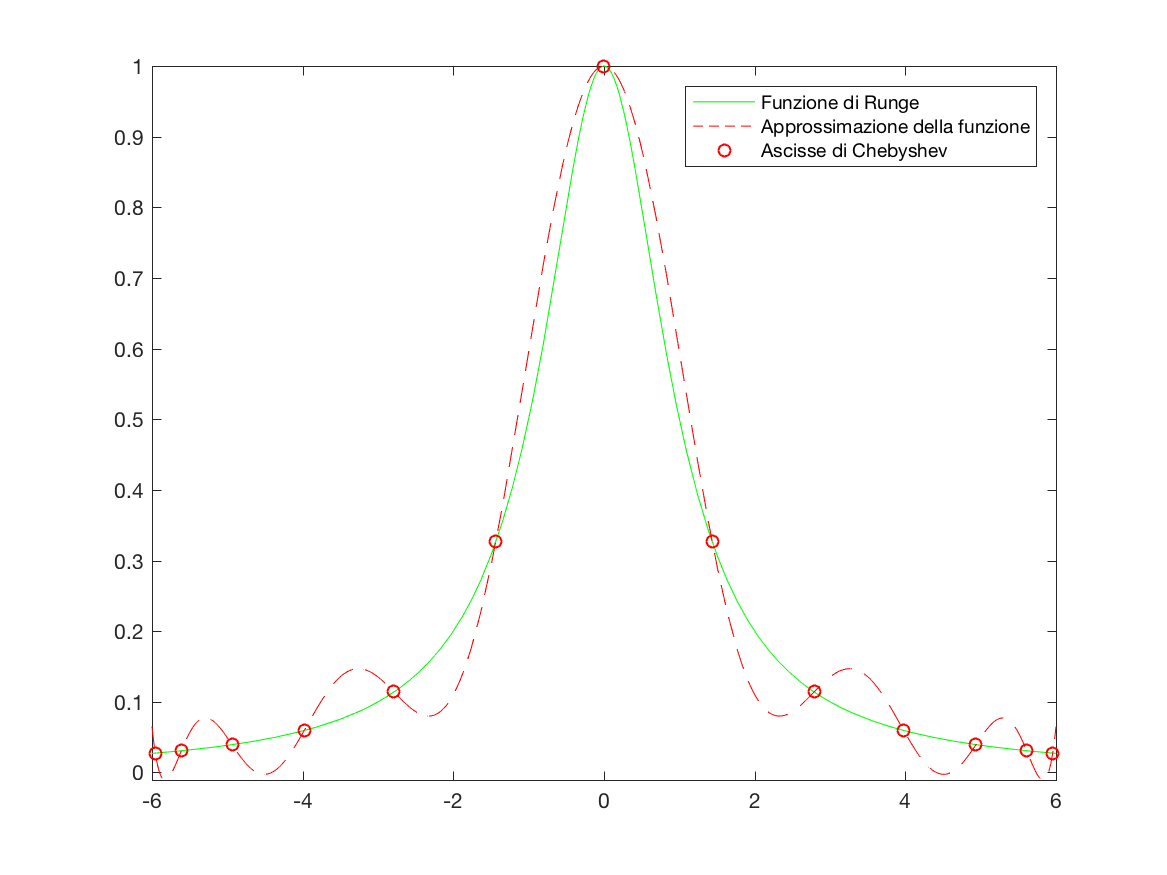
\includegraphics[scale=0.333]{Capitolo4/graficiEs7/es4_7_img12.png} \\
\end{tabular} \\
\noindent\begin{tabular}{c c}
\(n=16\) & \(n=22\) \\
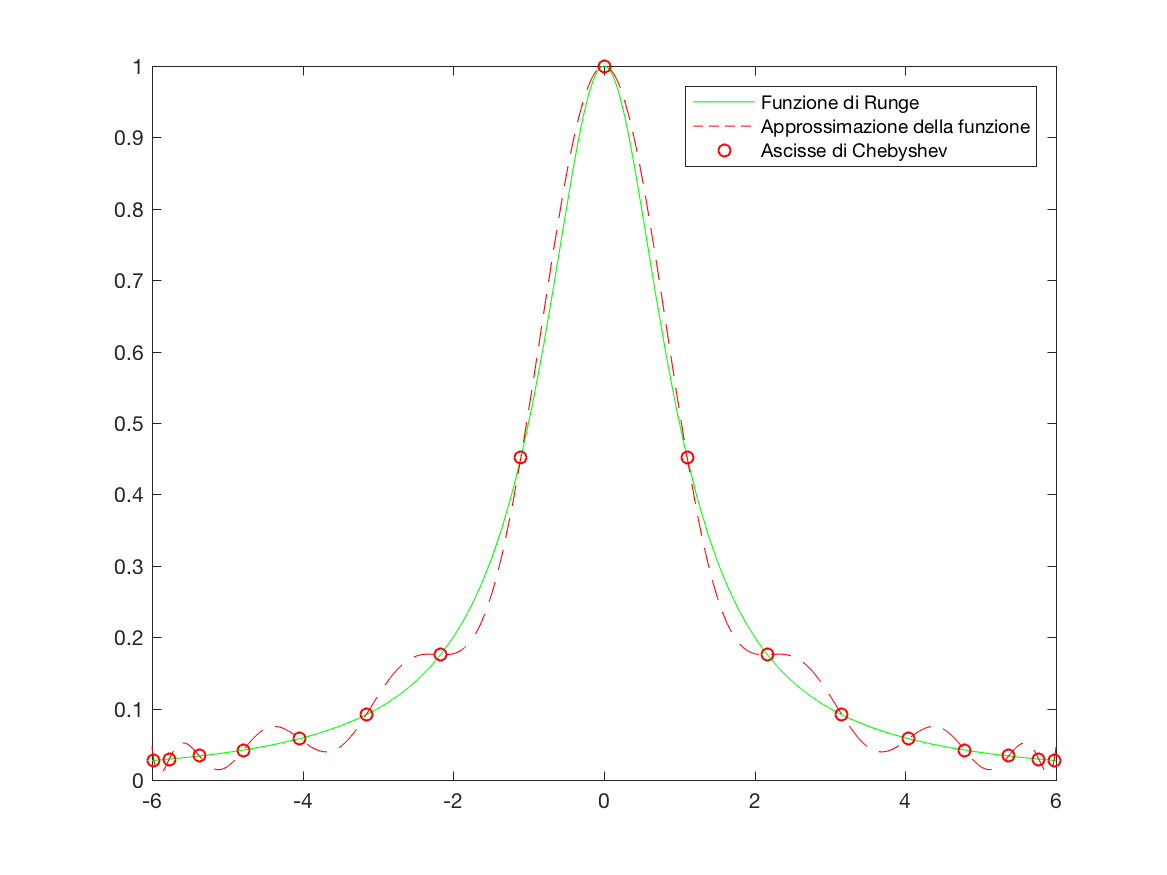
\includegraphics[scale=0.333]{Capitolo4/graficiEs7/es4_7_img16.png} &  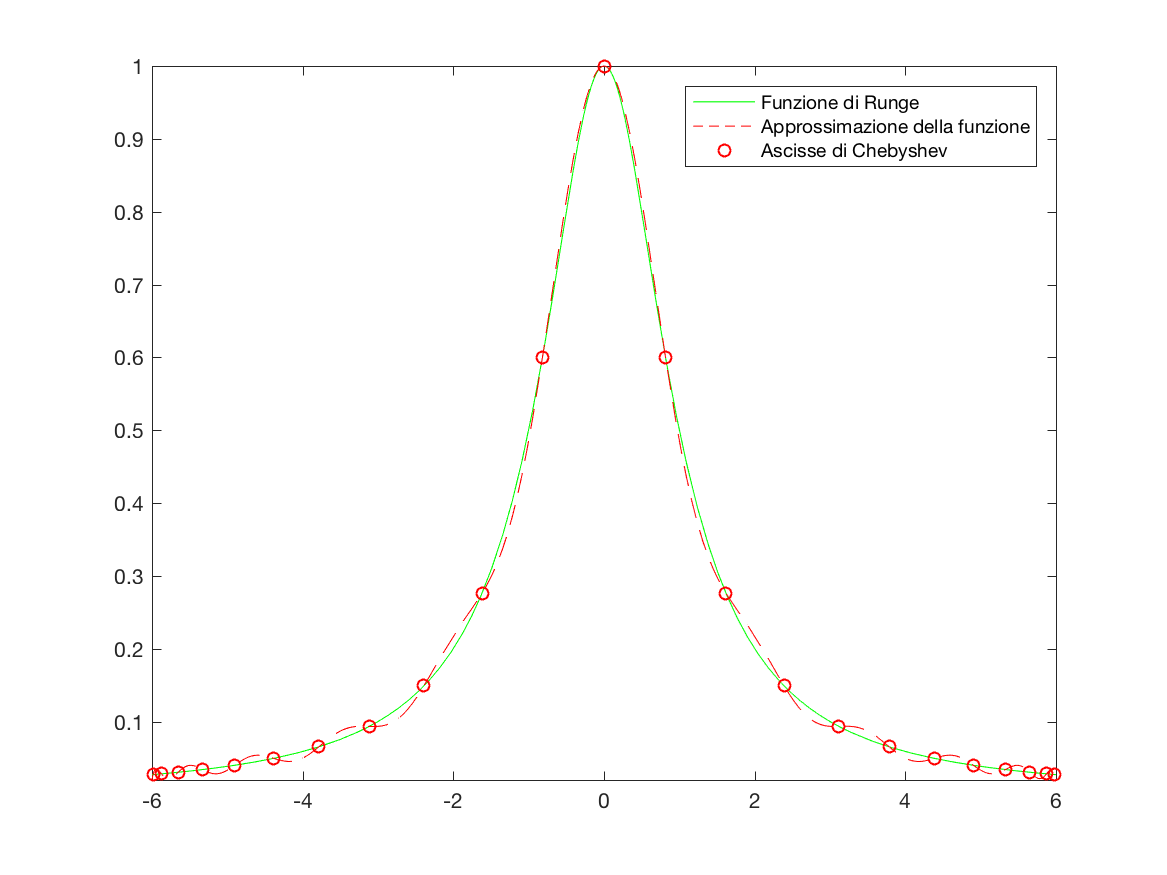
\includegraphics[scale=0.333]{Capitolo4/graficiEs7/es4_7_img22.png} \\
\(n=28\)& \(n=30\) \\
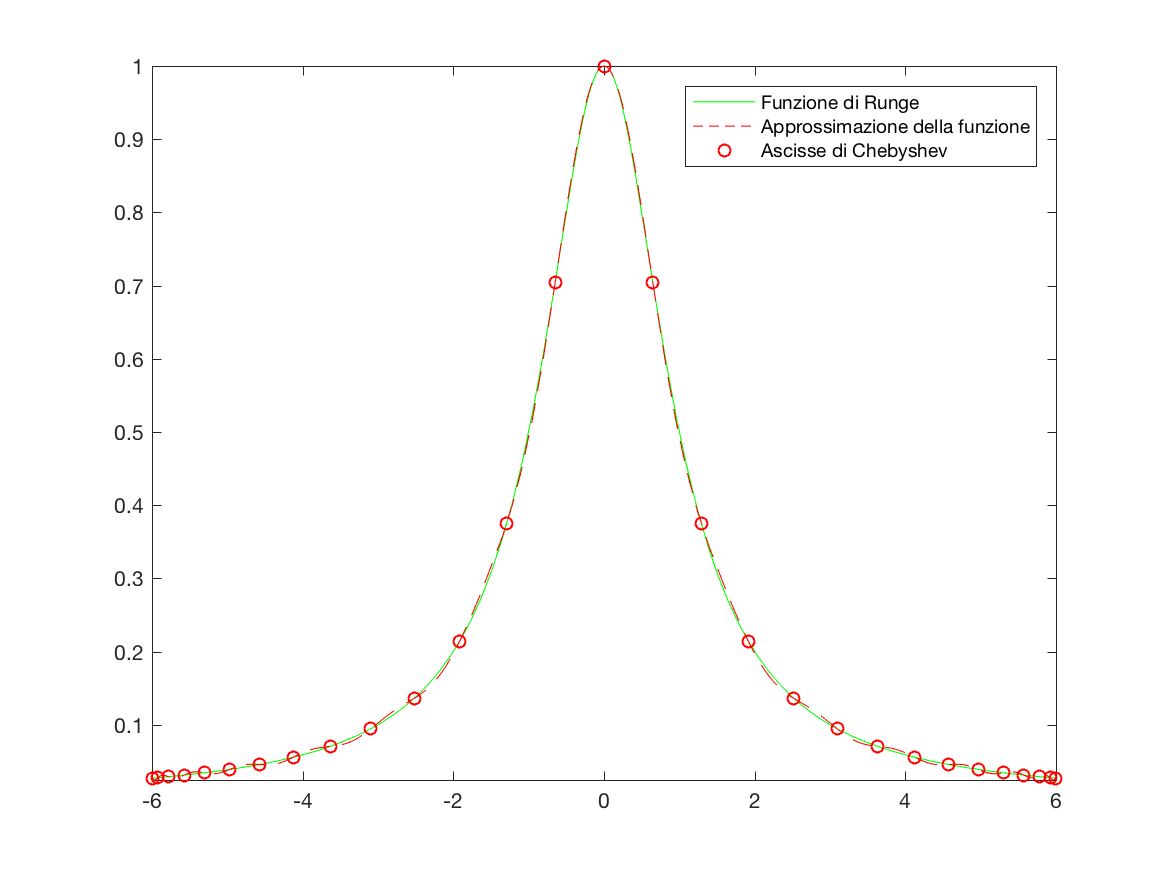
\includegraphics[scale=0.333]{Capitolo4/graficiEs7/es4_7_img28.png} &  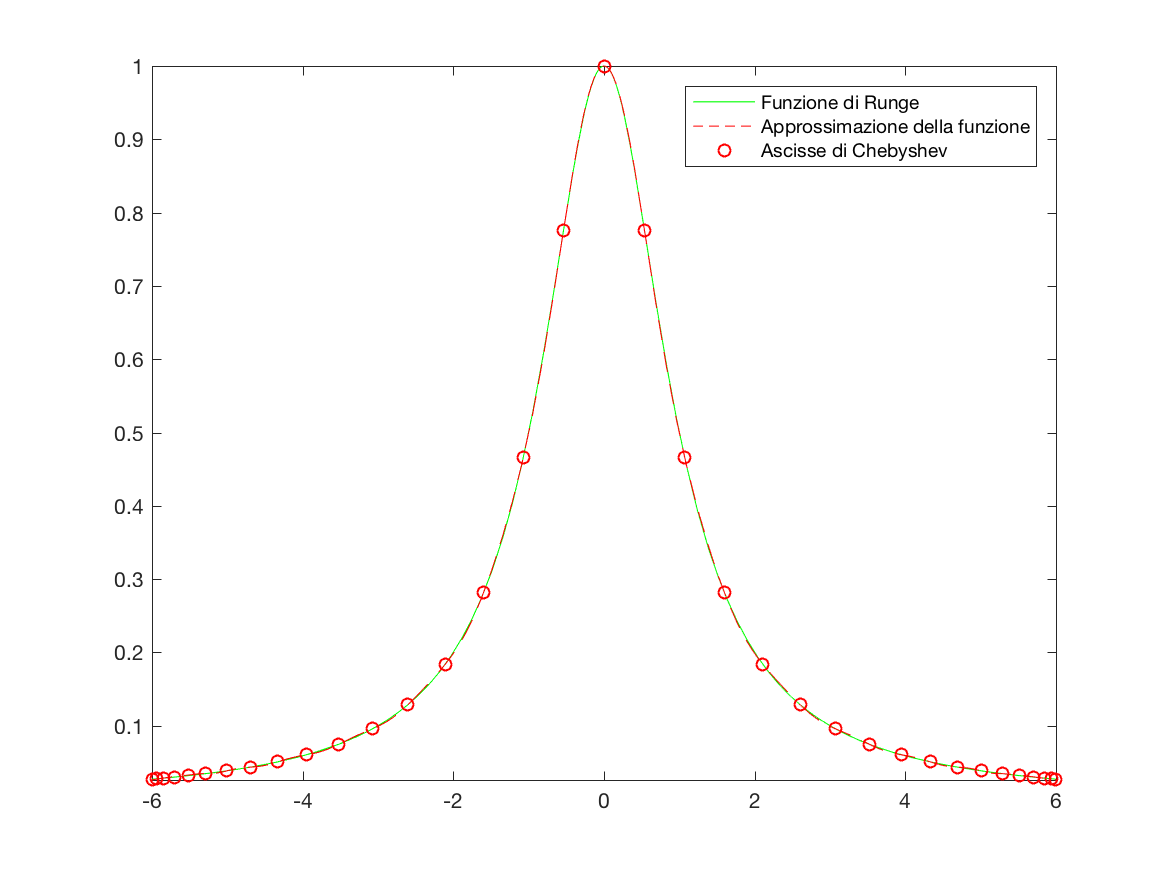
\includegraphics[scale=0.333]{Capitolo4/graficiEs7/es4_7_img34.png} \\
\(n=40\) &  \\
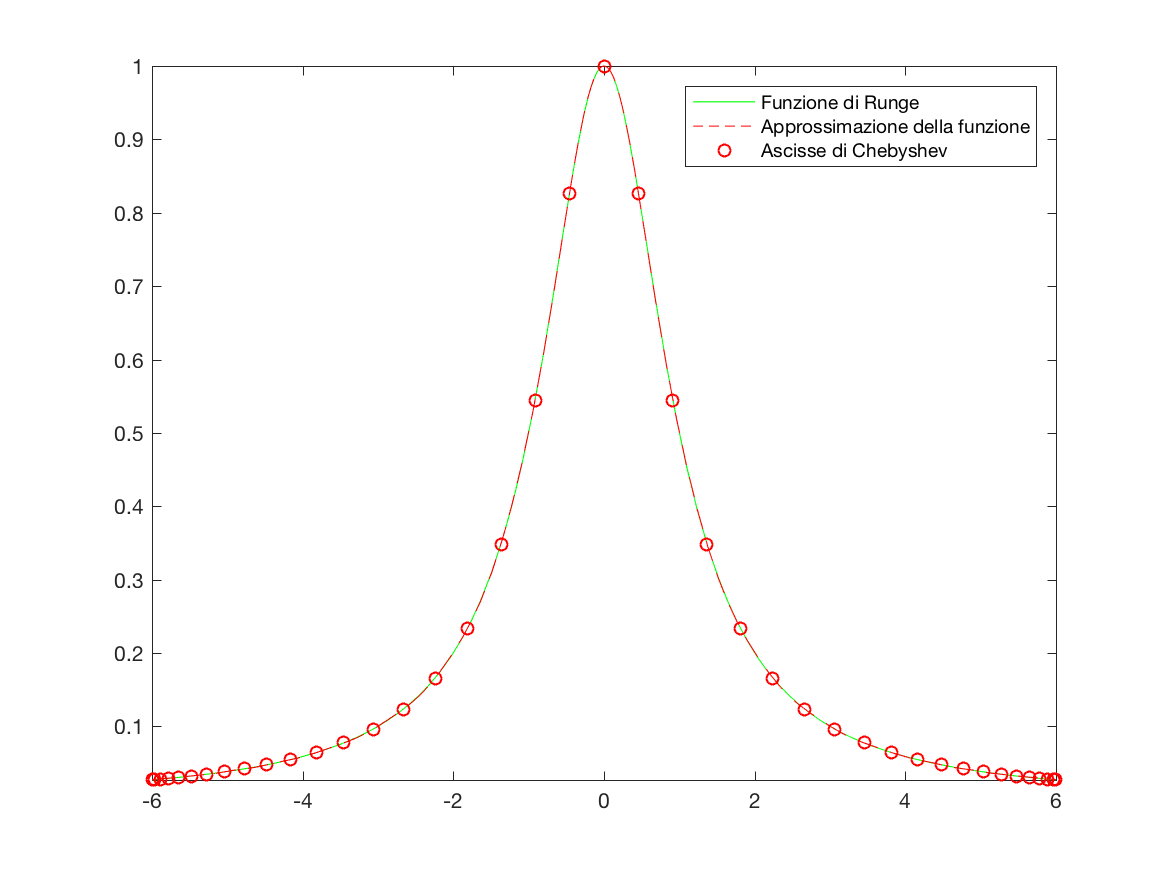
\includegraphics[scale=0.333]{Capitolo4/graficiEs7/es4_7_img40.png} &   \\
\end{tabular} \\
L'errore � stato calcolato seguendo la seguente formula:
$$
||e|| \approx ||f(x) - p_n(x)||_{\inf}
$$
Dove $f$ � intesa come la funzione di Runge e $p$ il suo polinomio interpolante.
\newpage
L'errore stimato � visibile nella seguente tabella:
\begin{center}
	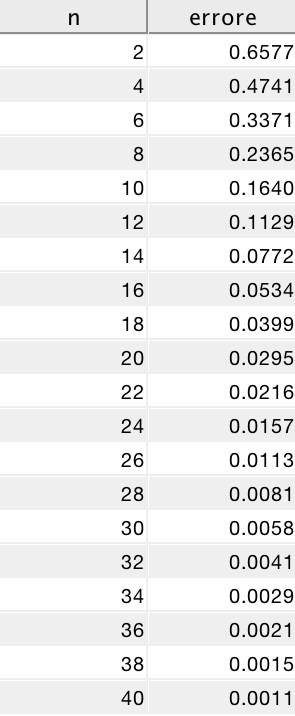
\includegraphics[scale=0.4]{Capitolo4/es4_7_tabErrore.png}
\end{center}
Notiamo che, utilizzando le ascisse di Chebyshev, aumentando il numero di punti otteniamo un'approssiamazione sempre pi� vicina alla funzione di Runge. Infatti l'errore diminuisce all'aumentare di n tendendo a 0 quando n tende all'infinito.

\bigskip
\textbf{Esercizio 4.8} \textit{Relativamente al precedente esercizio, stimare numericamente la crescita della costante di Lebesgue.}\\
\textbf{Soluzione: } La stima della costante di Lebesgue mediante le ascisse di Chebyshev � data dalla seguente formula:
\[
\Lambda_n \approx \frac{2}{\pi}\log n
\]
Ci si aspetta quindi che abbia una crescita logaritmica al crescere di \(n\).
\newpage
La tebella seguente  mette in evidenza tale comportamento:
\begin{center}
	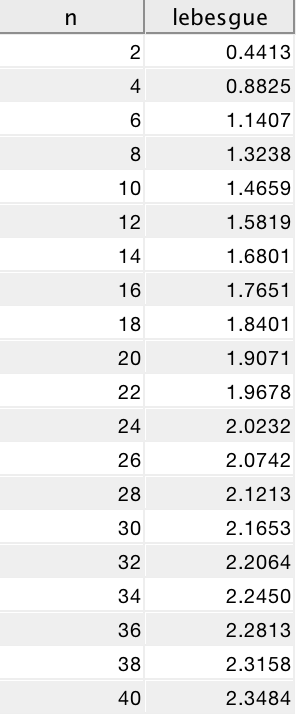
\includegraphics[scale=0.4]{Capitolo4/es4_8_tabella.png}
\end{center}

\bigskip
\textbf{Esercizio 4.9} \textit{Utilizzare la function ell'Esercizio 4.1 per approssimare la funzione di Runge sull'intervallo \([-6, 6]\), su una partizione uniforme di \(n+1\) ascisse per \(n = 2, 4, 6, \ldots, 40\). Stimare le corrispondenti costanti di Lebesgue.}\\
\textbf{Soluzione: }
\begin{tabular}{cc}
\(n=2\) & \(n=4\) \\
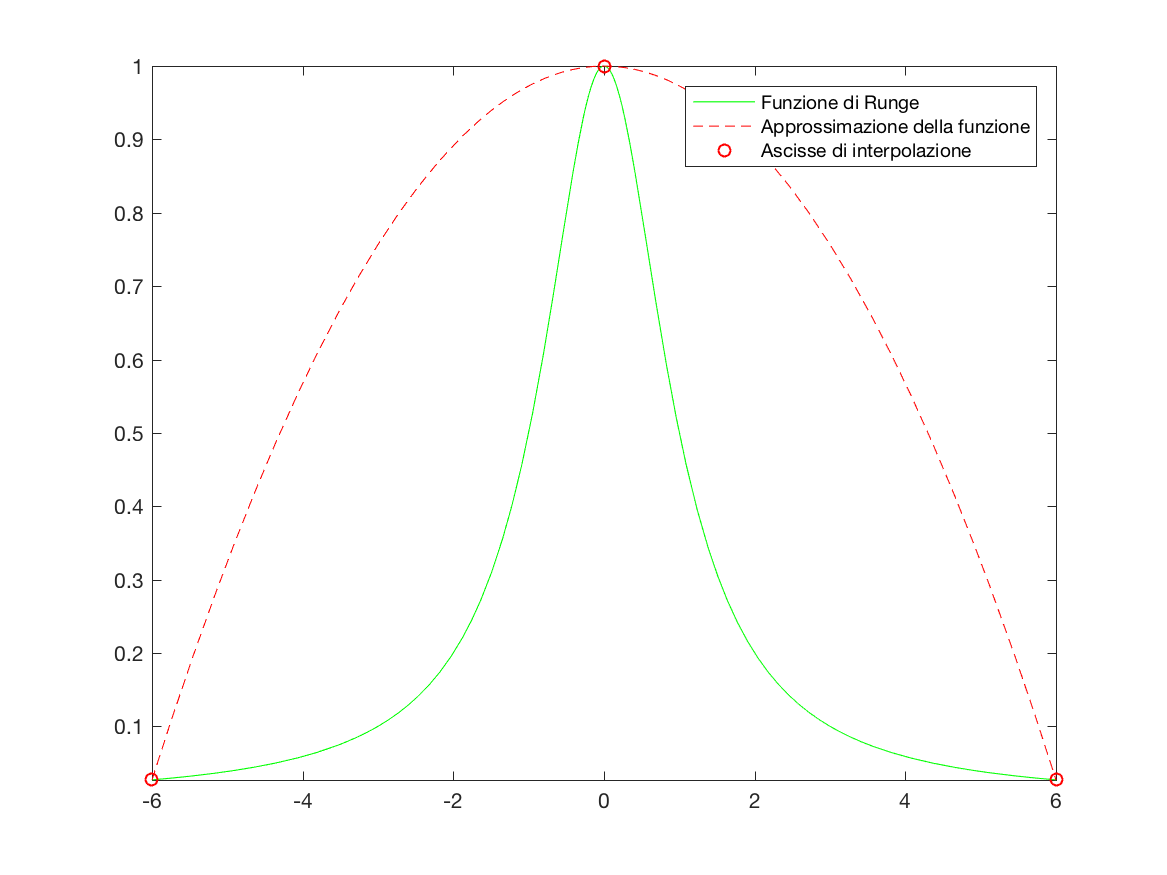
\includegraphics[scale=0.333]{Capitolo4/graficiEs9/es4_9_img2.png} &  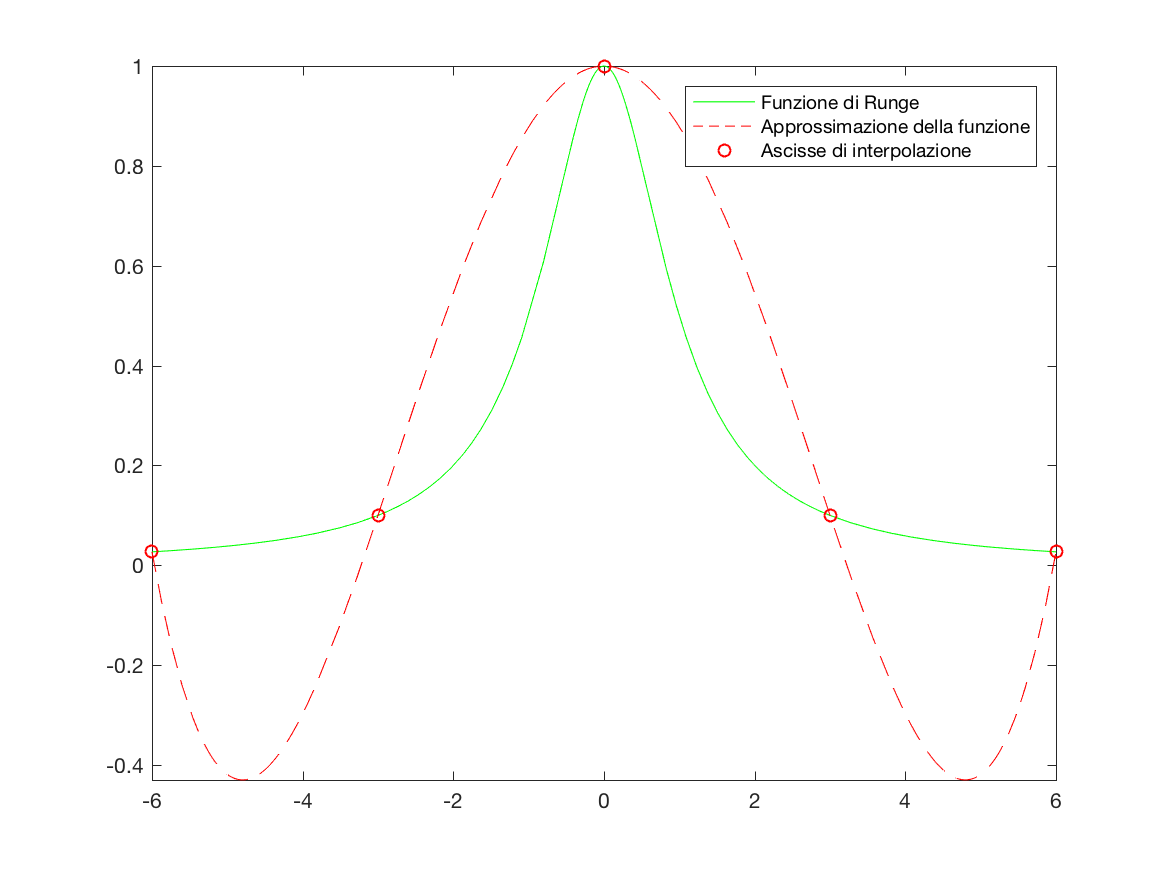
\includegraphics[scale=0.333]{Capitolo4/graficiEs9/es4_9_img4.png} \\
\end{tabular} \\
\begin{tabular}{cc}
\(n=6\) & \(n=8\) \\
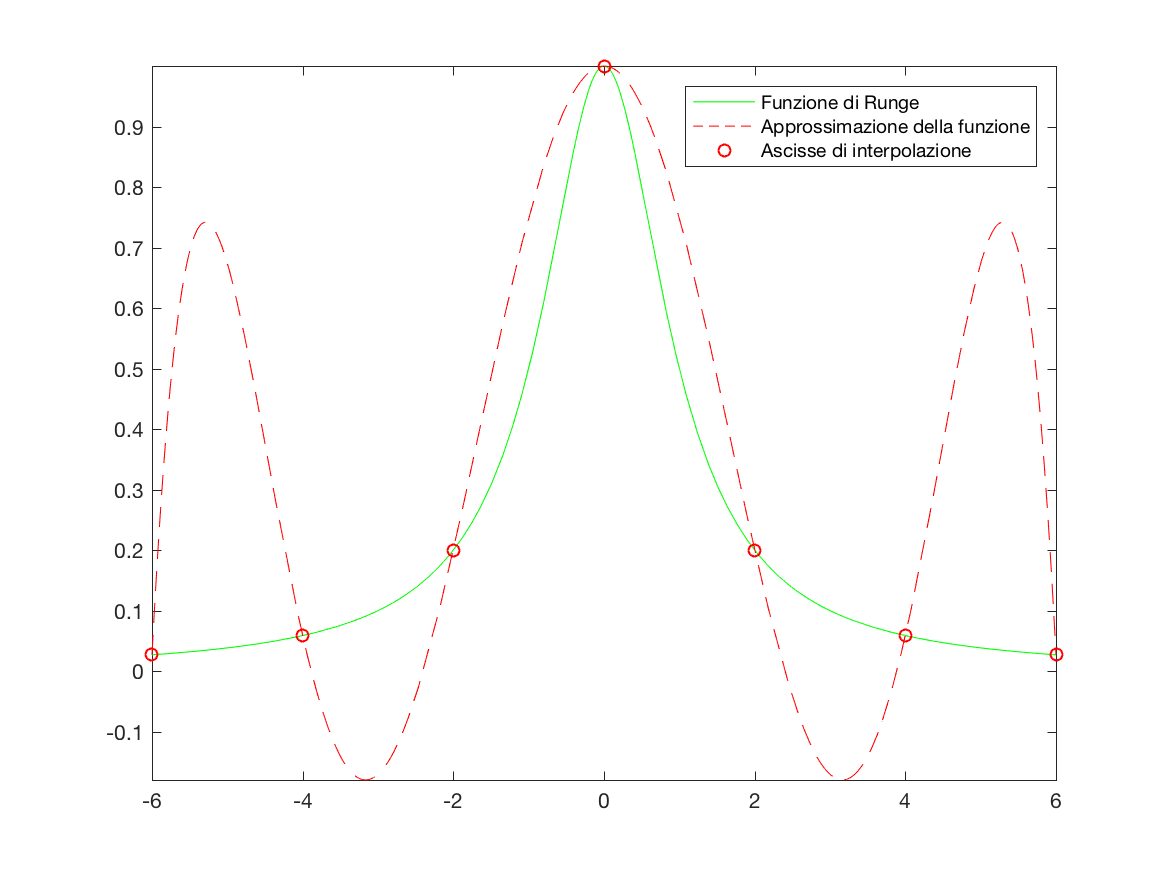
\includegraphics[scale=0.333]{Capitolo4/graficiEs9/es4_9_img6.png} &  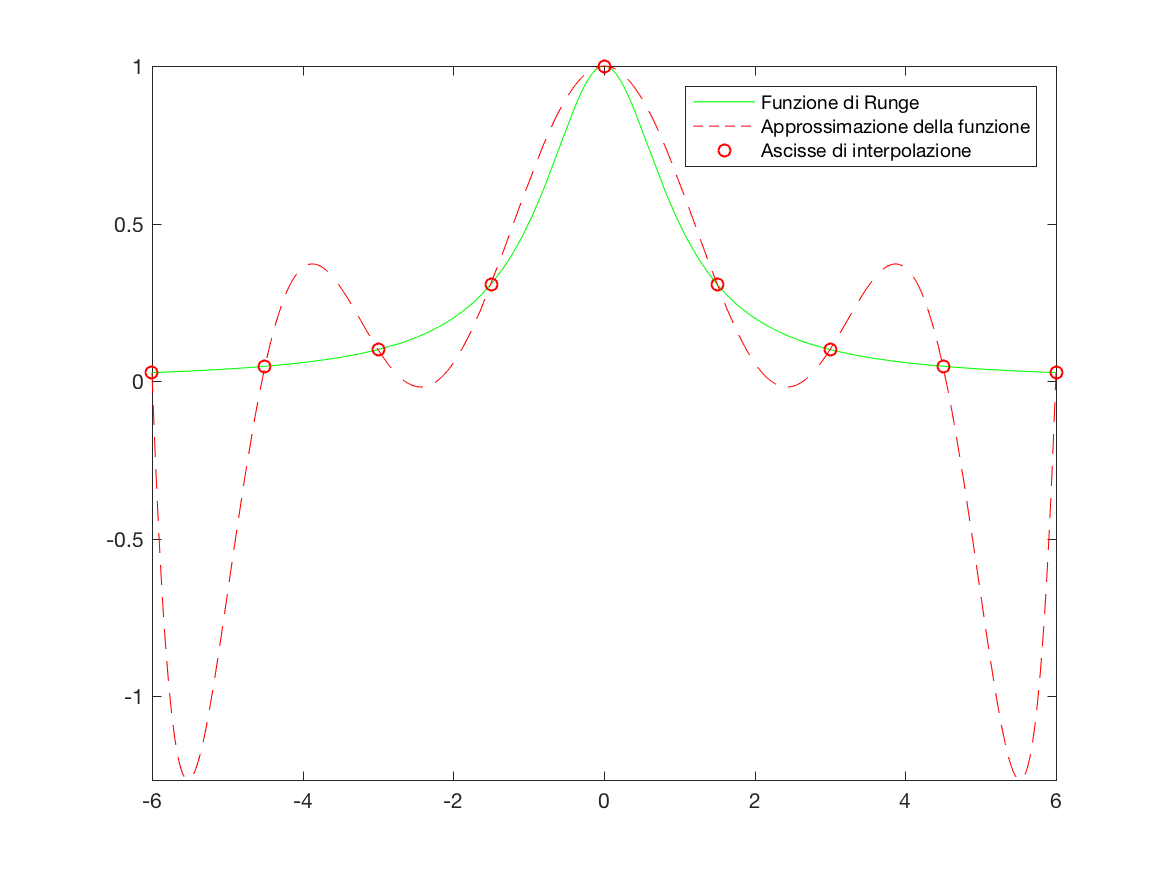
\includegraphics[scale=0.333]{Capitolo4/graficiEs9/es4_9_img8.png} \\
\(n=10\) & \(n=12\) \\
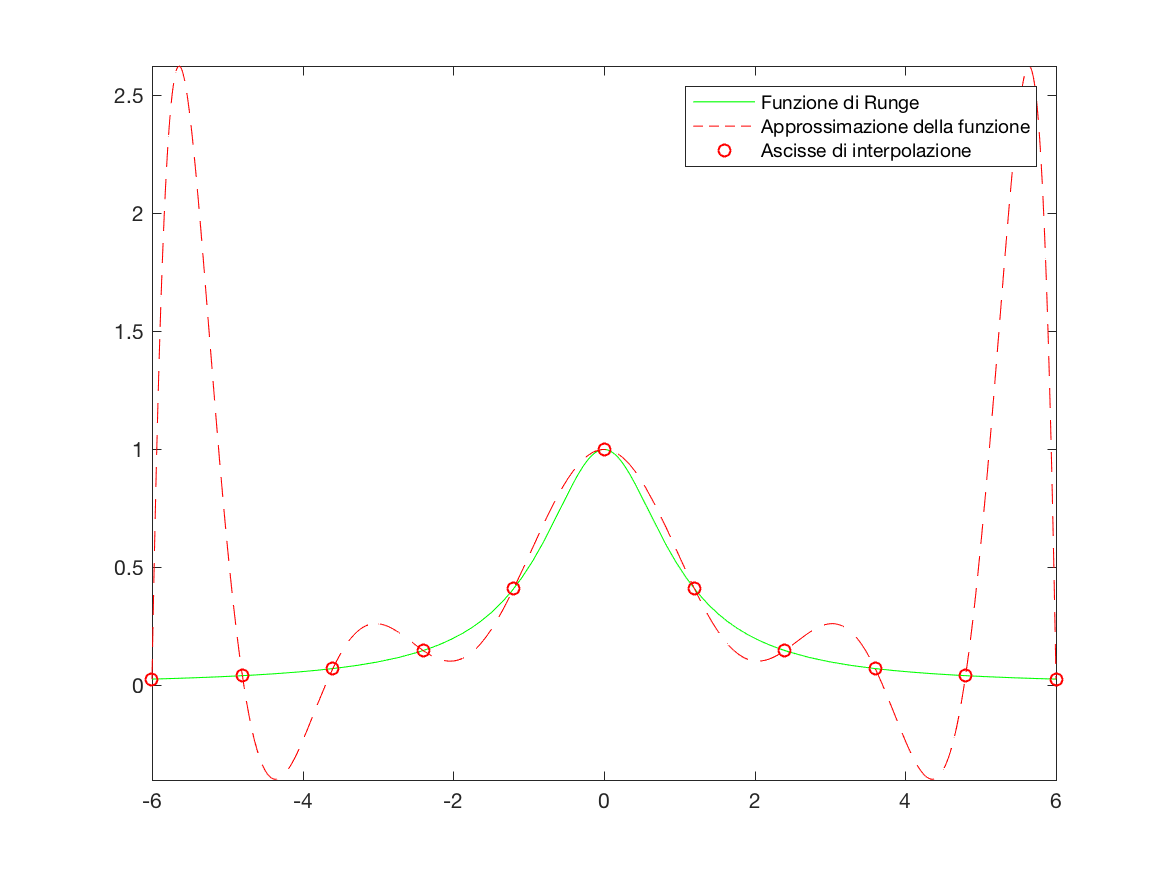
\includegraphics[scale=0.333]{Capitolo4/graficiEs9/es4_9_img10.png} &  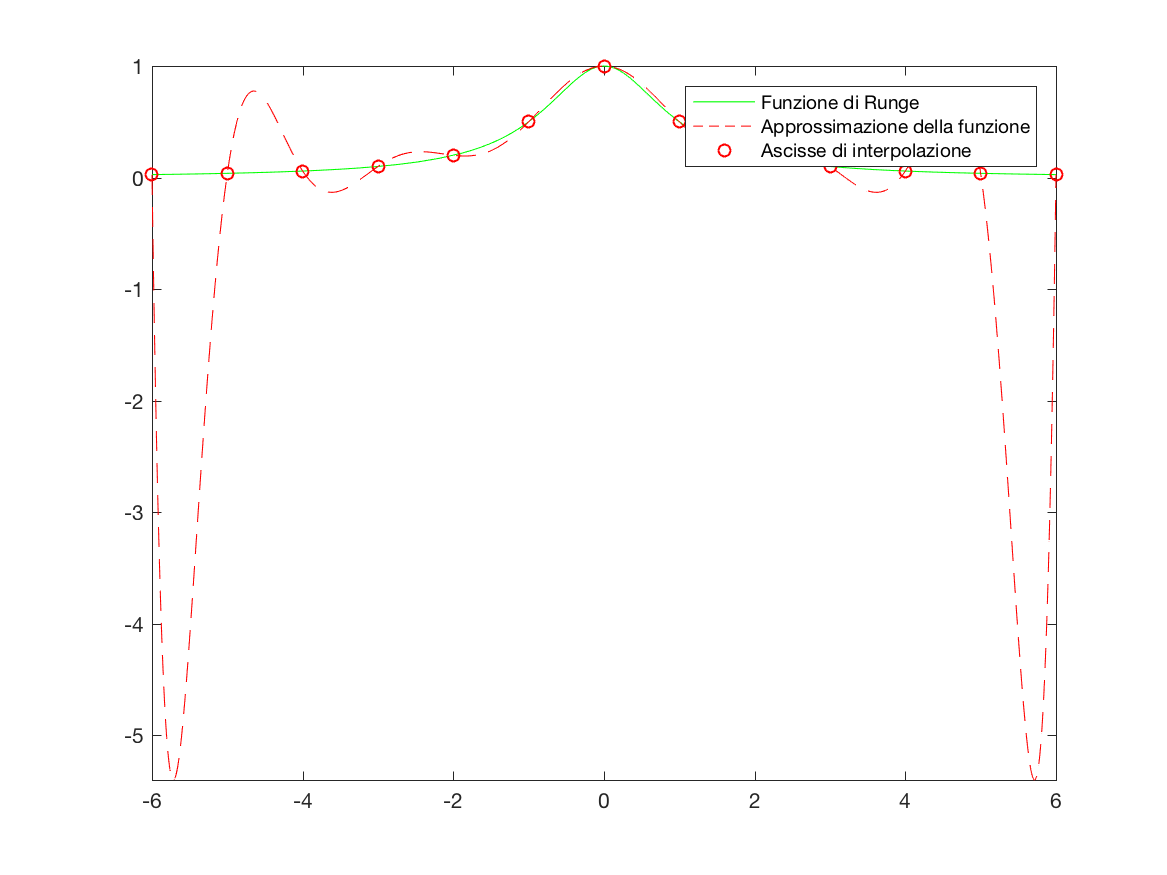
\includegraphics[scale=0.333]{Capitolo4/graficiEs9/es4_9_img12.png} \\
\(n=16\) & \(n=22\) \\
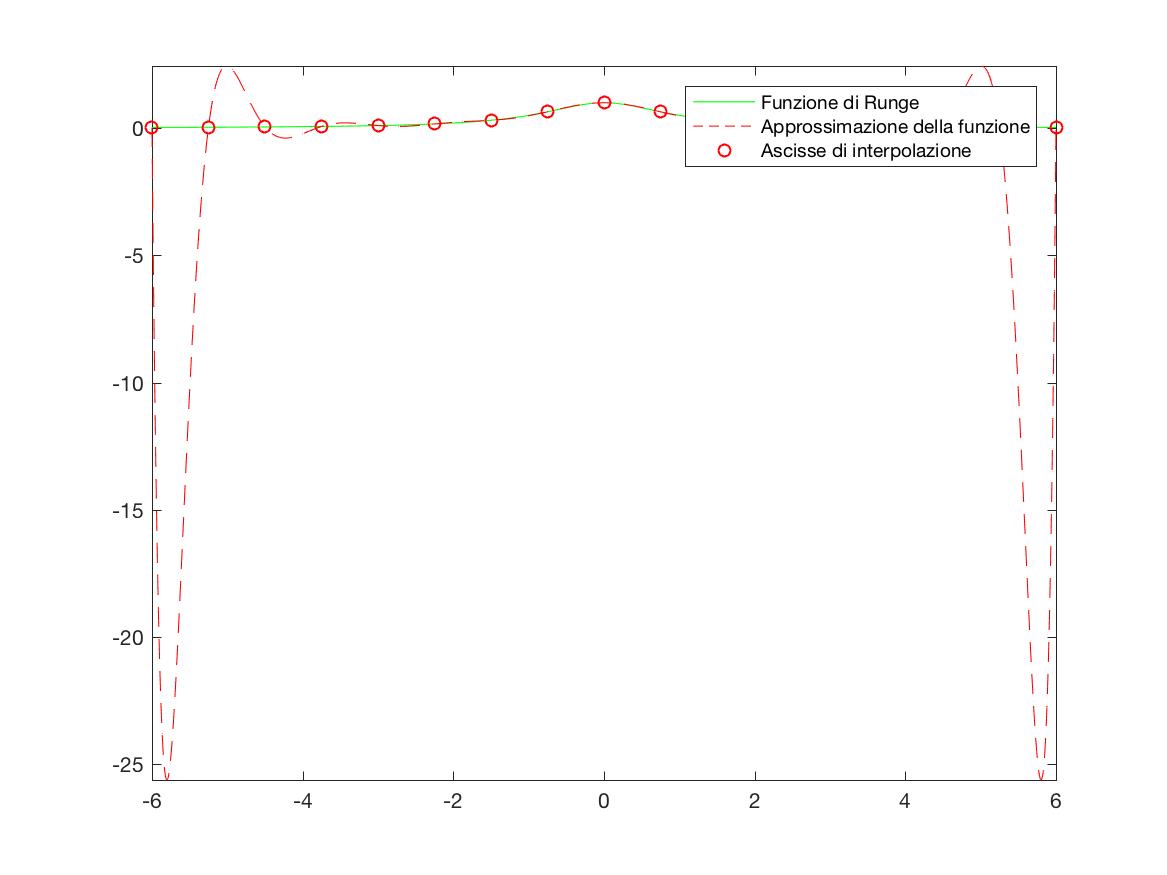
\includegraphics[scale=0.333]{Capitolo4/graficiEs9/es4_9_img16.png} &  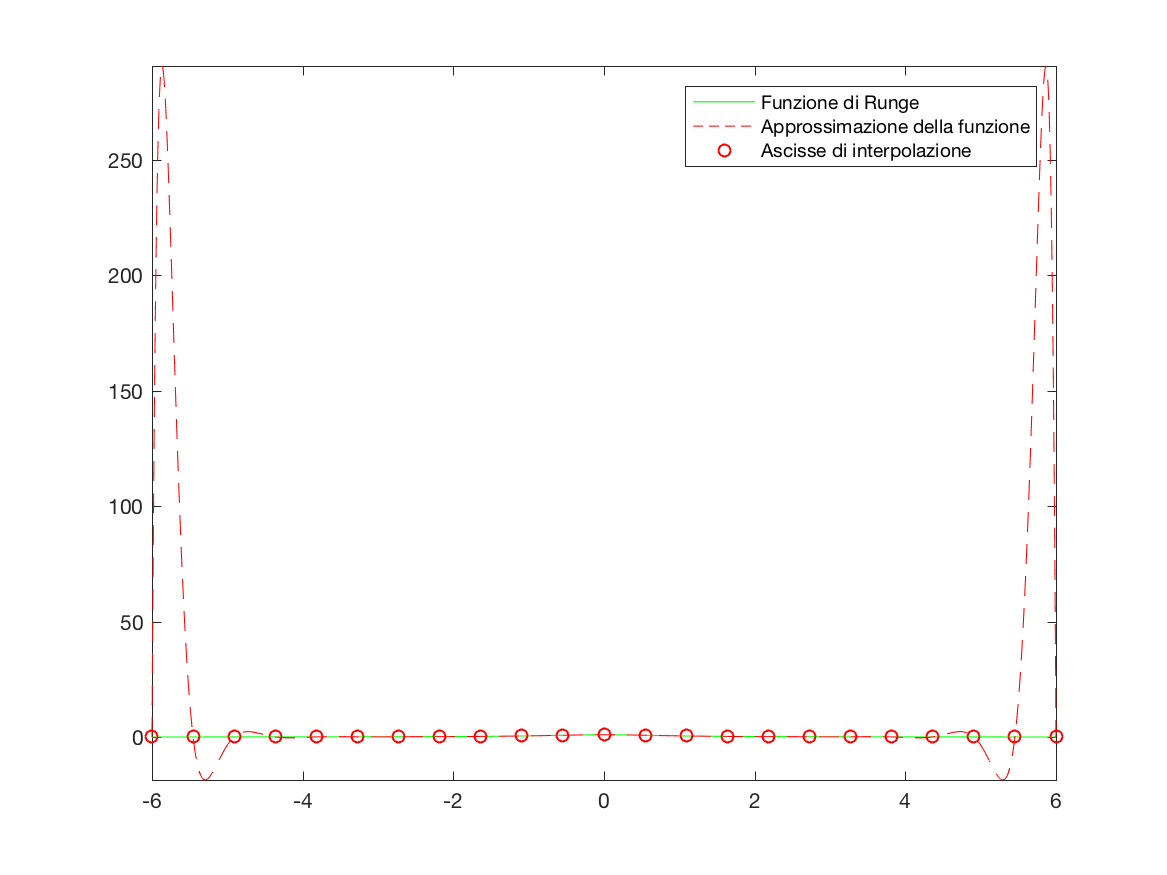
\includegraphics[scale=0.333]{Capitolo4/graficiEs9/es4_9_img22.png} \\
\end{tabular} \\
\begin{tabular}{cc}
\(n=28\) & \(n=34\) \\
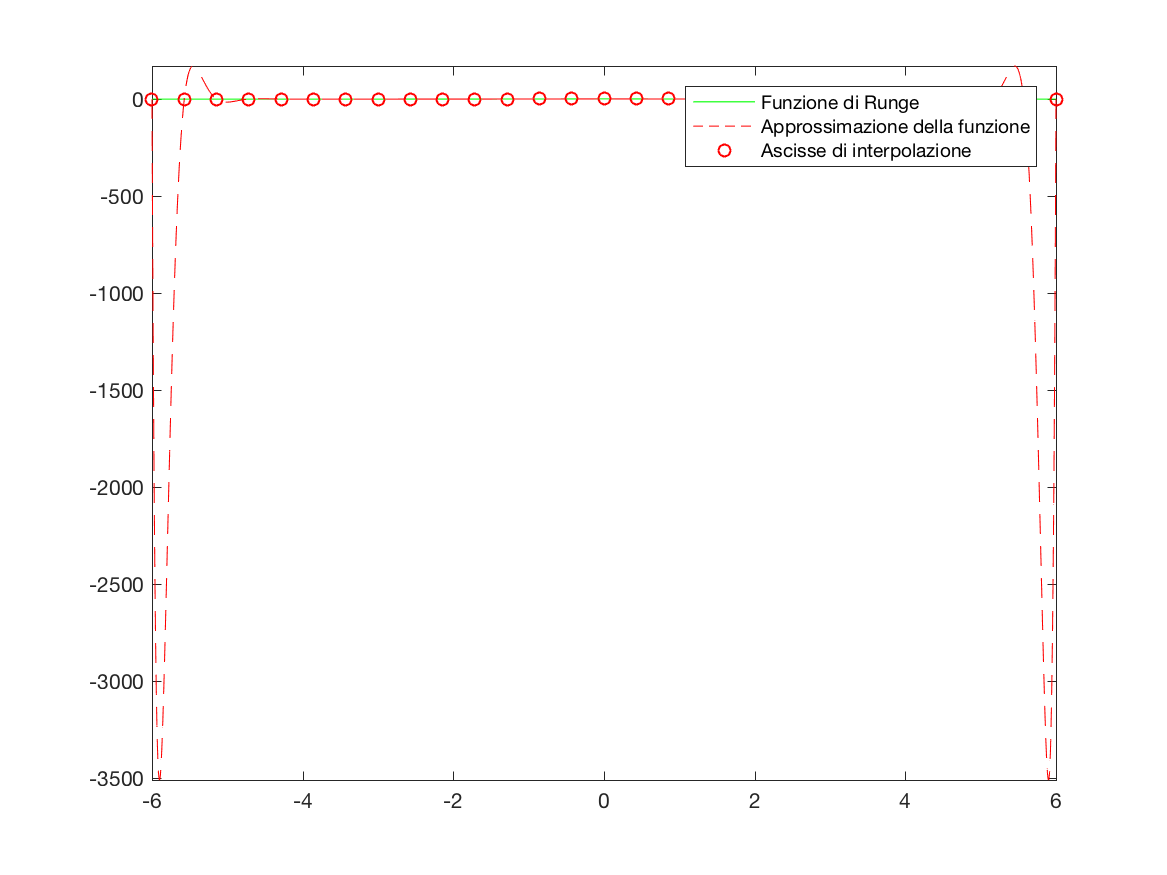
\includegraphics[scale=0.333]{Capitolo4/graficiEs9/es4_9_img28.png} &  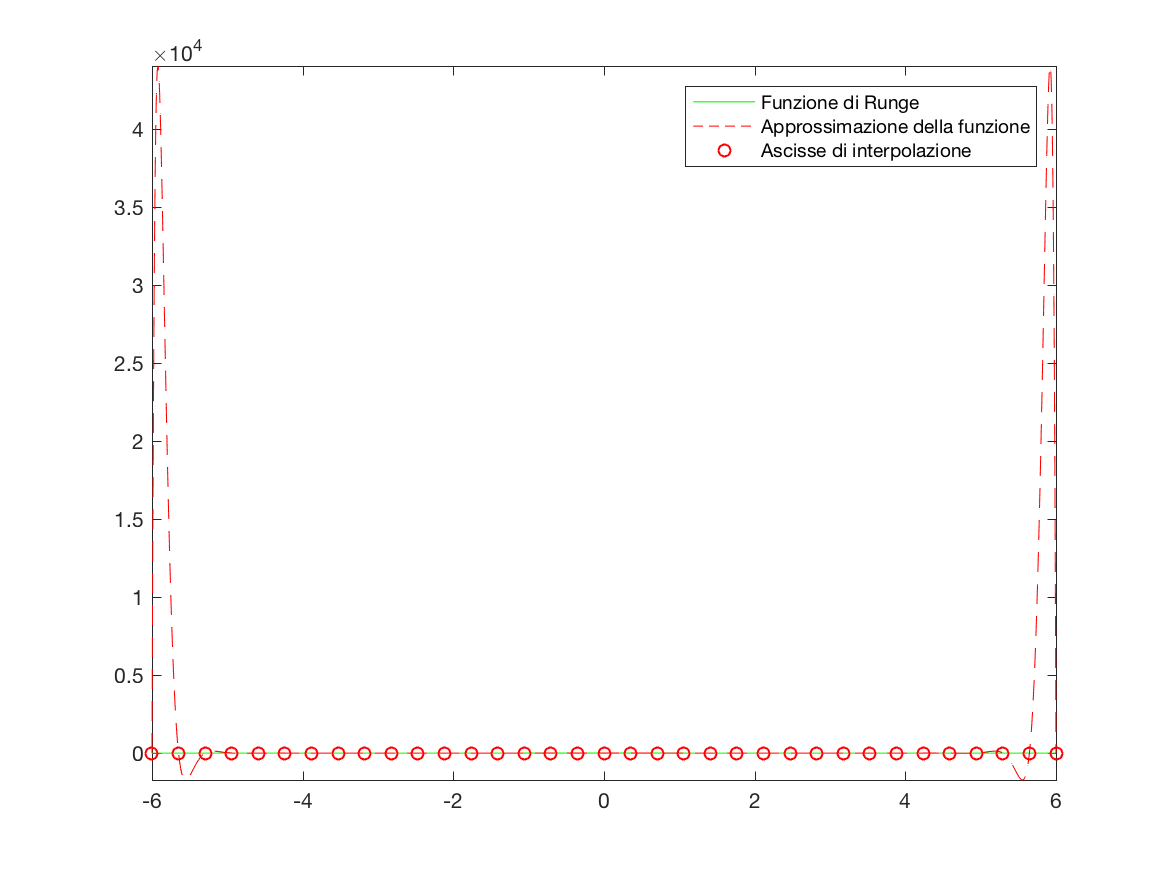
\includegraphics[scale=0.333]{Capitolo4/graficiEs9/es4_9_img34.png} \\
\(n=40\) &  \\
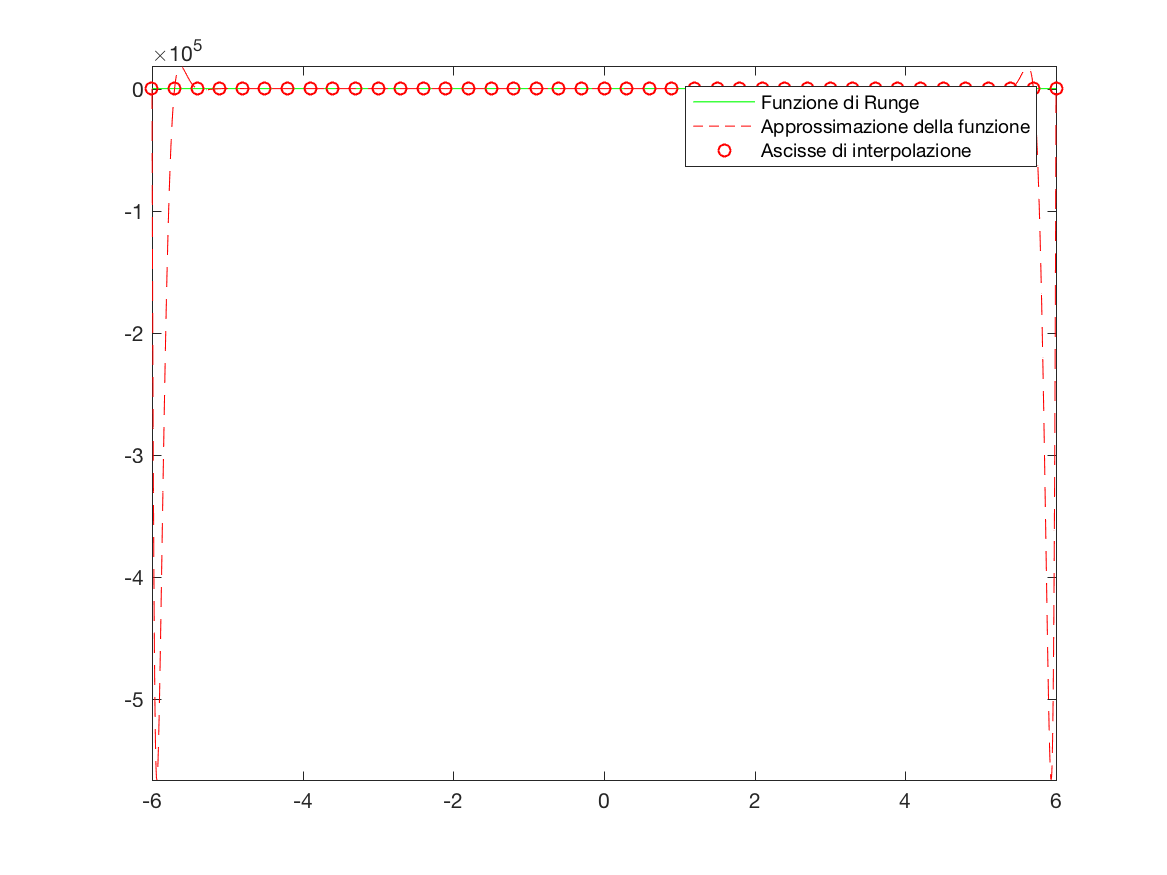
\includegraphics[scale=0.333]{Capitolo4/graficiEs9/es4_9_img40.png} &  \\
\end{tabular} \\
Di seguito riportiamo la tabella con le stime degli errori e della costante di Lebesgue in funzione del grado n:
\begin{center}
	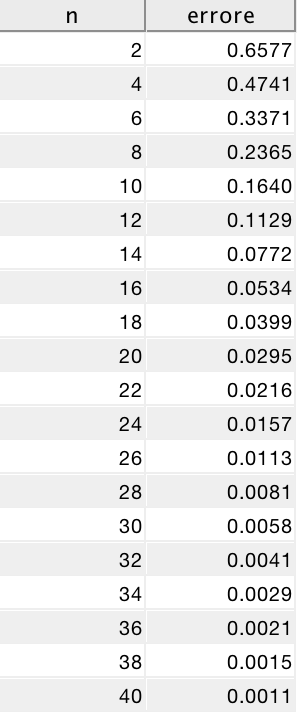
\includegraphics[scale=0.333]{Capitolo4/es4_9_tabella.png}
\end{center}
\bigskip
\textbf{Esercizio 4.10} \textit{Stimare, nel senso dei minimi quadrati, posizione, velocit� iniziale ed accelerazione relative ad un moto rettilineo uniformemente accelerato per cui sono note le seguenti misurazioni dele coppie (tempo, spazio):\\
\((1, 2.9) \quad (1, 3.1)\quad (2, 6.9) \quad (2, 7.1) \quad (3, 12.9) \quad (3, 13.1) \quad (4, 20.9) \quad (4, 21.1)\)\\\((5, 30.9) \quad (5, 31.1)\)}\\
\textbf{Soluzione: }Il problema posto consiste nel risolvere\\
\[
y = s(t) = x_{0} + v_{0}t + \frac{1}{2}at^{2}, \qquad \text{con } a, x_{0} \text{ e } v_{0} \text{ costanti}
\]
La stima, nel senso dei minimi quadrati, equivale alla risoluzione del sistema lineare sovradeterminato Ax=b:
\[
\begin{pmatrix}1 & 1 & 1 \\ 1 & 1 & 1 \\ 1 & 2 & 4 \\ 1 & 2 & 4 \\ 1 & 3 & 9 \\ 1 & 3 & 9 \\ 1 & 4 & 16 \\ 1 & 4 & 16 \\ 1 & 5 & 25 \\ 1 & 5 & 25 \end{pmatrix} \begin{pmatrix}x \\ v \\  a/2\end{pmatrix} = \begin{pmatrix} 2.9\\3.1\\6.9\\7.1\\12.9\\13.1\\20.9\\21.1\\30.9\\31.1 \end{pmatrix}
\]
Il problema � ben posto ed esiste un'unica soluzione in quanot abbiamo misurazioni in $n+1$ ascisse.\\
La matrice A � una matrice di Vandermonde con rango massimo 3. \\
\'E possibile calcolare una soluzione per il sistema dato utilizzando le function per la risoluzione e fattorizzazione dei sistemi QR sviluppati negli eserci precedenti:
\[
\begin{pmatrix}x\\v\\a/2 \end{pmatrix} = \begin{pmatrix}1\\1\\0.99999\end{pmatrix}
\]
\end{flushleft}

\chapter{Esercizi A.A. 2017-18}
\markboth{CAPITOLO 5. ESERCIZI A.A. 2017-18}{CAPITOLO 5. ESERCIZI A.A. 2017-18}
\begin{flushleft}
\textbf{Esercizio 5.1} \textit{Scrivere una function Matlab che implementi la formula composita dei trapezi su \(n+1\) ascisse equidistanti nell'intervallo \([a, b]\) relativamente alla funzione implementata da \lstinline[language=Matlab]{Capitolo5/fun(x)}.\\La function deve essere del tipo \lstinline[language=Matlab]{Capitolo5/If = trapcomp(a, b, fun, tol)}.}\\
\textbf{Soluzione: }\lstinputlisting[language=Matlab]{Capitolo5/es5_1.m}
\bigskip
\textbf{Esercizio 5.2} \textit{Scrivere una function Matlab che implementi la formula composita di Simpson su \(2n+1\) ascisse equidistanti nell'intervallo \([a, b,]\) relativamente alla funzione implementata da \lstinline[language=Matlab]{Capitolo5/fun(x)}.\\La function deve essere del tipo \lstinline[language=Matlab]{Capitolo5/If = simpcomp(a, b, fun, tol)}.}\\
\textbf{Soluzione: }\lstinputlisting[language=Matlab]{Capitolo5/es5_2.m}
\bigskip
\textbf{Esercizio 5.3} \textit{Scrivere una function Matlab che implementi la formula composita dei trapezi adattativa nell'intervallo \([a, b]\) relativamente alla funzione implementata da \lstinline[language=Matlab]{Capitolo5/fun(x)} e con tolleranza \lstinline[language=Matlab]{Capitolo5/tol}.\\La function deve essere del tipo \lstinline[language=Matlab]{Capitolo5/If = trapad(a, b, fun, tol)}.}\\
\textbf{Soluzione: }\lstinputlisting[language=Matlab]{Capitolo5/es5_3.m}
\bigskip
\textbf{Esercizio 5.4} \textit{Scrivere una function Matlab che implementi la formula composita di Simpson adattativa nell'intervallo \([a, b]\) relativamente alla funzione implementata da \lstinline[language=Matlab]{Capitolo5/fun(x)} e con tolleranza \lstinline[language=Matlab]{Capitolo5/tol}.\\La function deve essere del tipo \lstinline[language=Matlab]{Capitolo5/If = simpad(a, b, fun, tol)}.}\\
\textbf{Soluzione: }\lstinputlisting[language=Matlab]{Capitolo5/es5_4.m}
\bigskip
\textbf{Esercizio 5.5} \textit{Calcolare quante valutazioni di funzione sono necessarie per ottenere una approssimazione di
\[I(f) = \int_0^1 \exp(-10^6 x) dx \]
che vale $10^{-6}$ in doppia precisione IEEE, con una tolleranza $10^{-9}$, utilizzando le functions dei precedenti esercizi. Argomentare quantitativamente la risposta.}\\
\textbf{Soluzione:} Le functions degli esercizi precedenti esercizi sono state leggermente modificate e sono stati calcolati i seguenti valori:\\
\[
\begin{tabular}{l*{15}{c}}
	Function & \vline & Valutazioni & \vline & Errore \\
	\hline
	Trapezi composita & \vline & 10000001 & \vline & $8.3319 \times 10^{-10}$ \\
	Simpson composita & \vline & 2000002 & \vline & $3.3715 \times 10^{-10}$ \\
	Trapezi adattiva & \vline & 77823 & \vline & $1.1252 \times 10^{-14}$\\
	Simpson adattiva & \vline & 1038 & \vline & $1.6469 \times 10^{-14}$\\
\end{tabular}
\]
Possiamo vedere che per la funzione presa in esame performano meglio le formule adattive in quanto individuano i nodi della partizione in base al comportamento locale della funzione, questo permette di minimizzare l'errore e di raggiungere la soglia di tolleranza prestabilita.\\
Viceversa le formule con ascisse equispaziate si sono rilevate inadeguate per questo tipo di funzione che presenta una rapida variazione di valore in una porzione dell'intervallo molto ristretta.\\
Il codice utilizzato per ottenere i risultati posti sopra:
\lstinputlisting[language=Matlab]{Capitolo5/es5_5.m}
\end{flushleft}

\chapter{Esercizi A.A. 2017-18}
\markboth{CAPITOLO 6. ESERCIZI A.A. 2017-18}{CAPITOLO 6. ESERCIZI A.A. 2017-18}
\begin{flushleft}

\bigskip
\textbf{Esercizio 6.1} \textit{Scrivere una function Matlab che generi la matrice \textit{sparsa} $n \times n$, con $n > 10$\\
$$
A_n = \begin{pmatrix} a_{11} & \ldots & a_{1n} \\ \vdots & & \vdots \\ a_{n1} & \ldots & a_{nn}\end{pmatrix}, \qquad \text {con } \qquad a_{ij} \begin{cases} 4 \text{ se } i = j \\ -1 \text{ se } i = j \pm 1 \\ -1 \text{ se } i = j \pm 10\end{cases}
$$
Utilizzare a questo fine la function Matlab \lstinline{spdiags}.}\\
\textbf{Soluzione: }
\lstinputlisting[language=Matlab]{Capitolo6/es6_1.m}
\bigskip
\textbf{Esercizio 6.2} \textit{	Utilizzare il metodo delle potenze per calcolare l'autovalore dominante della matrice $A_n$ del precedente esercizio, con una approssimazione $tol=10^{-5}$, partendo da un vettore con elementi costanti. Riempire, quindi, la seguente tabella: \\ \begin{center}
\begin{tabular}{ | l | c | r |}
	\hline
	$n$ & \textit{numero iterazioni effettuate} & \textit{stima autovalore} \\ \hline
	100 &  &  \\ \hline
	\vdots &  &  \\  \hline
1000 &  &  \\
	\hline
\end{tabular}
\end{center}}
\textbf{Soluzione: }La tabella richiesta � la seguente:\\
\[
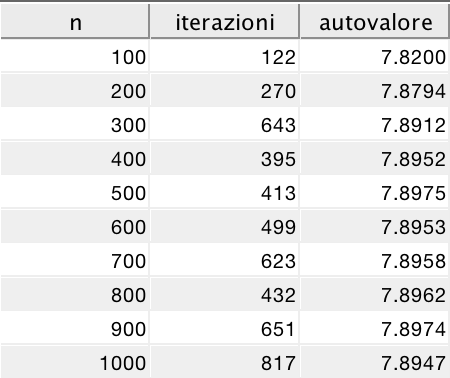
\includegraphics[scale=0.4]{Capitolo6/es6_2.png}
\]
Generata grazie al seguente codice matlab:
\lstinputlisting[language=Matlab]{Capitolo6/es6_2.m}
\newpage
\textbf{Esercizio 6.3} \textit{	Utilizzare il metodo di Jacobi per risolvere il sistema lineare\\
	\[
	A_n \textbf{x} = \begin{pmatrix} 1 \\ \vdots \\ 1 \end{pmatrix},
	\]
	dove $A_n$ � la matrice definita in (1), con tolleranza $tol=10^{-5}$, e partendo dal vettore nullo. Graficare il numero di iterazioni necessarie, rispetto alla dimensione $n$ del problema, con $n$ che varia da 100 a 1000 (con passo 20).}\\
\textbf{Soluzione: }
\[
	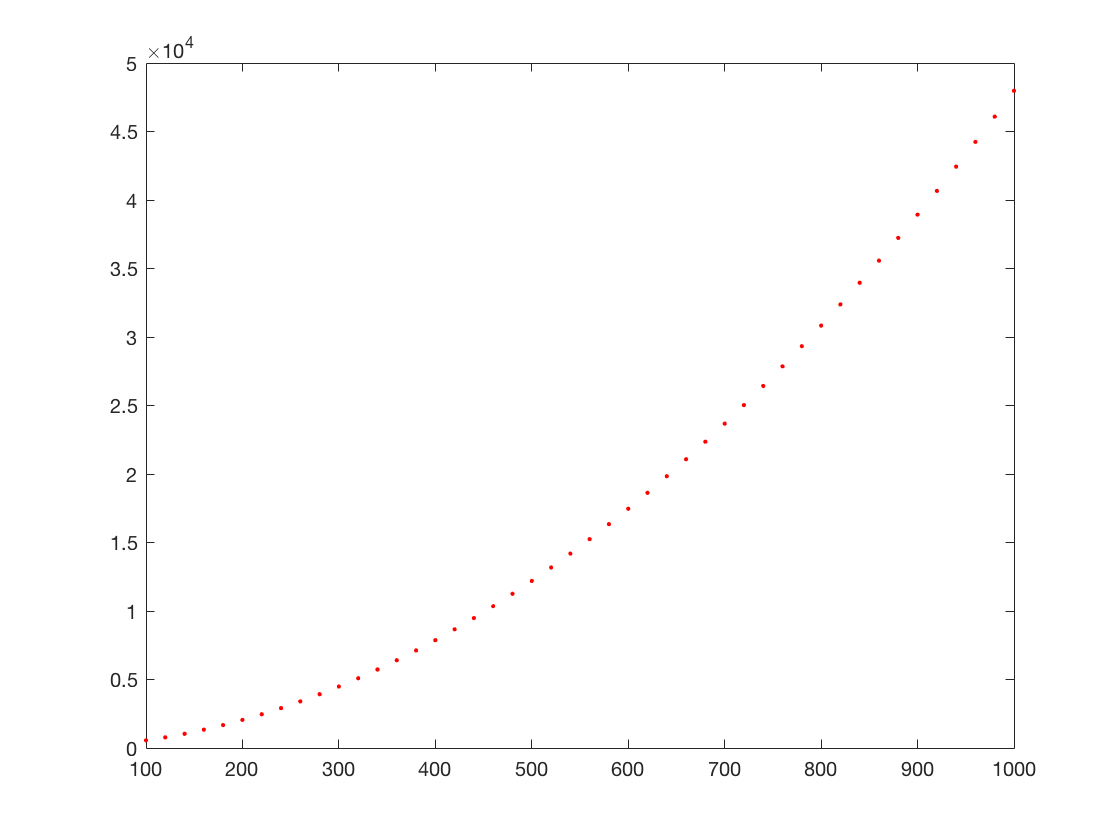
\includegraphics[scale=0.35]{Capitolo6/es6_3.png}
\]
Il codice matlab che ha generato il grafico:
\lstinputlisting[language=Matlab]{Capitolo6/es6_3.m}

\bigskip
\textbf{Esercizio 6.4} \textit{ Ripetere una procedura analoiga a quella del precedente esercizio utilizzando il metodo di Gauss-Seidel.}\\
\textbf{Soluzione: }
\[
	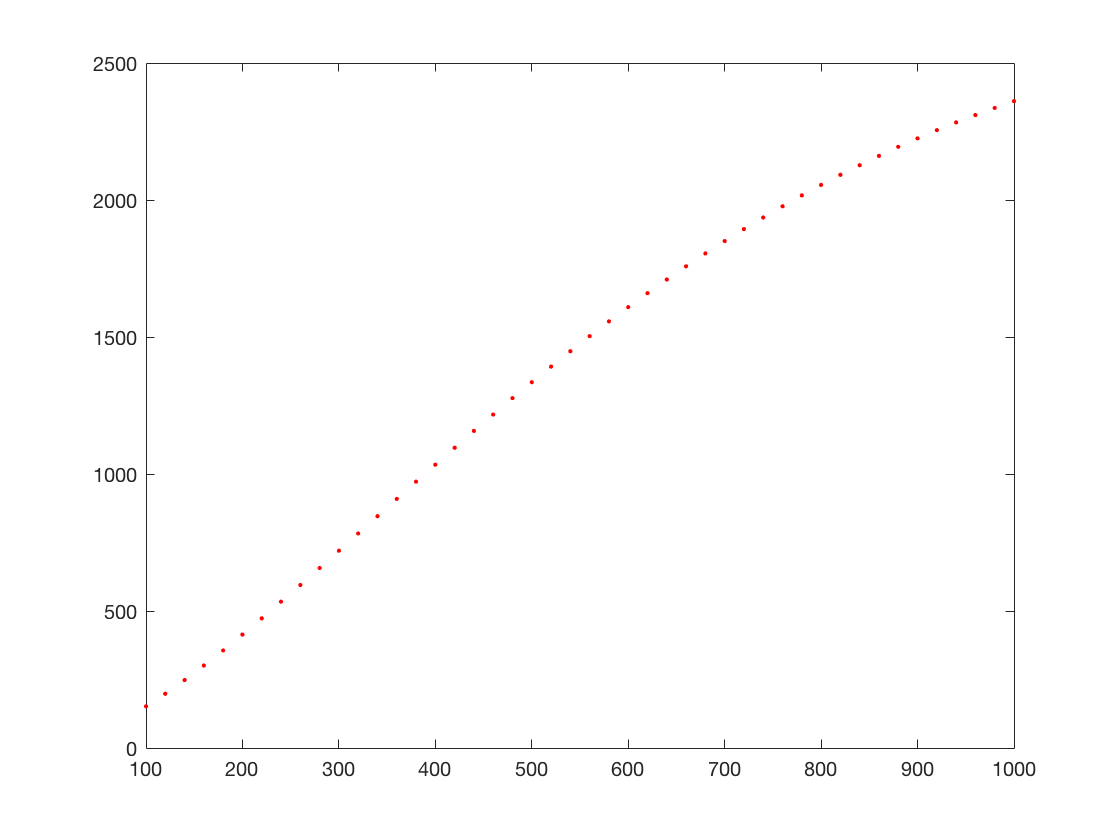
\includegraphics[scale=0.35]{Capitolo6/es6_4.png}
\]
Il codice matlab che ha generato il grafico:
\lstinputlisting[language=Matlab]{Capitolo6/es6_4.m}
\newpage
\textbf{Esercizio 6.5} \textit{
Con riferimento al sistema lineare (2), con $n=1000$, graficare la norma dei residui rispetto all'indice di iterazione, generati dai metodi di Jacobi e Gauss-Seidel. Utilizzare il formato \lstinline{semilogy} per realizzare il grafico, corredandolo di opportune $label$.}
\textbf{Soluzione: }
Il seguente grafico � realizzato con le ascisse in scala logaritmica tramite il formato semilogaritmico semilogy di Matlab:
\[
	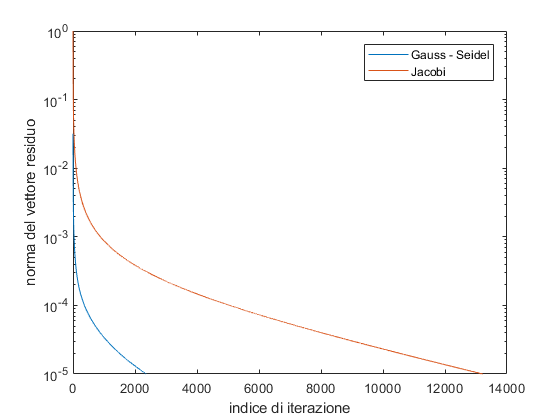
\includegraphics[scale=0.85]{Capitolo6/es6_5.png}
\]
Il codice matlab che ha generato il grafico:
\lstinputlisting[language=Matlab]{Capitolo6/es6_5.m}

\end{flushleft}


\end{document}
